\documentclass[main]{subfiles}

\begin{document}
% Chapter Template
\setcounter{chapter}{2}

% Controllers
%  Uncoupled sinusoidal oscillators
%  Chaotic systems
%  Chua Circuit
%   Simple limiter control in Mathematica
\chapter{Controllers} % Main chapter title

\label{Chapter\thechapter} % Change X to a consecutive number; for referencing this chapter elsewhere, use \ref{ChapterX}

\lhead{Chapter \thechapter. \emph{Controllers}} % Change X to a consecutive number; this is for the header on each page - perhaps a shortened title

\section{Adaptive controllers for locomotion}
%% rev. 1

Starting in the industrial revolution, people have started to automatize production and thereby lowered the costs of production of almost any good. Today's production robots can perform very sophisticated manipulation as is required for large-scale products such as cars of smaller scale products such as electronic chips. However, the most efficient robots to date are robots specifically built for the task at hand. Many of them work in cages without interaction with humans and totally lack autonomy or adaptability, even though the morphology could theoretically be reused for another task. But since task does not require any learning, adaption or autonomous behavior, it is not programmed to do so. As more recent developments strive for more autonomy and adaptivity in robots, more adaptable controllers need to be developed. Tasks requiring autonomy and adaptivity are rescue, detection or exploration scenarios of robots performing outdoor. Such a task is generally very versatile, as it is totally unknown what situation has to be expected and what problems will have to be solved. This means that problems have to be solved in a much more robust manner than it has to be done in a supervised environment, because the situation could change. Also the importance of low latency control arises because the system has to be reactive to its environment and is only in rare cases able to plan its movements far ahead. The requirements for such a controller therefore are to be highly adaptive on one hand and to control with very low latency on the other hand. Many different approaches to control exist, [?], however most of them are highly engineered approaches, so they suffer from high power and latency because traditional problem solving generally includes proper planning.  When compared to nature, these approaches are far from competitive. An ant for example can leave its nest, go out into the unknown, find food and communicate with other ants to collaboratively bring it back to the nest. This highly complex task requires a variety of skills, from perception and and classification to locomotion and manipulation of objects. Given that the ant has about 250'000 neurons [], the control output is highly complex, adaptive and comes with low latency. A subset of these neurons is responsible for the locomotion of the animal. But how can complex locomotion arise from a very simple controller? Could it be that multiple uncoupled controllers for different limbs can generate complex, robust locomotion patterns just by featuring periodic control signals? This would be a counterexample to the hypothesis that only very complex controllers can generate to complex gaits. Let us examine two different types of controllers, one non-adaptive sinusoidally oscillating controller and one adaptive chaotic controller.

\section{Uncoupled sinusoidal oscillators}
\label{sec:sinusoidal-oscillators}

First the non-adaptive controller was used to check if the evolutionary optimization is able to come up with solutions of a high enough variety in order to find valuable creature controller solutions to make a creature locomote on a flat terrain. The controller is fully distributed within the body of the creature and runs completely uncoordinated. It consists of many subcontrollers, whereas one subcontroller controls one degree of freedom in a certain joint. The controller's output is a simple sinusoidal signal defined by the parameters of amplitude and frequency and the X and Y offset in signal space. The parameter ranges are $\text{amplitude} \in [0,0.5]$, $\text{frequency} \in [0.1,4]$, $\text{offset}_X \in [0,2\Pi]$ and $\text{offset}_Y \in [0,1]$. Every time a Morphogene branch defining a joint is mutated, the sinusoidal subcontroller gets randomly initialized as well. The sinusoidal signal was then fed into a PID position controller to make the limb precisely follow the sinusoidal signal. Thereby the controller's solution is basically a set of sinusoids, that when applied to the co-evolved morphology results in a locomotion behavior that moves the creature forward. 

\section{Chaotic systems}

\lipsum[2]
\todo[inline]{Give a brief introduction to chaos theory.}

\subsection{Chua Circuit}
\label{subsec:chua-circuit}

According to \ref{bib:Kennedy1993}, for a circuit with time-varying output and no time-varying input that is built from electronic components such as resistors, capacitor and inductors, three criteria must hold in order to display chaotic behavior. It must contain:
  \begin{enumerate}
  \item at least one nonlinear element (where piecewise linear is sufficient)
  \item at least one locally active resistor
  \item at least three energy-storage elements
  \end{enumerate}
  
The simplest electronic circuit that satisfies these criteria is the Chua Circuit. Chua's circuit is chaotic system that can be built in the form of a simple electronic circuit. It was invented by Leon O. Chua when he visited the Waseda University in Japan in 1983. The circuit can be seen as a nonperiodic oscillator, that differently from an ordinary electronic oscillator never repeats its waveform. The circuit, remarkable because of its simplicity and rich variety of bifurcations and the presence of chaotic behavior, is one of the few physical systems for which the presence of chaos has been proven mathematically [again Kennedy1993].

\begin{figure}[H]
\centering
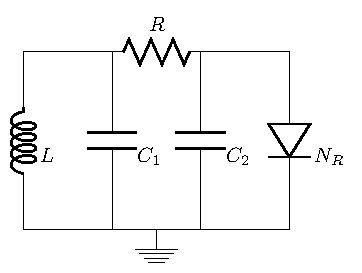
\includegraphics[width=0.49\textwidth]{chua-circuit/Chua-circuit-with-chua-diode.pdf}
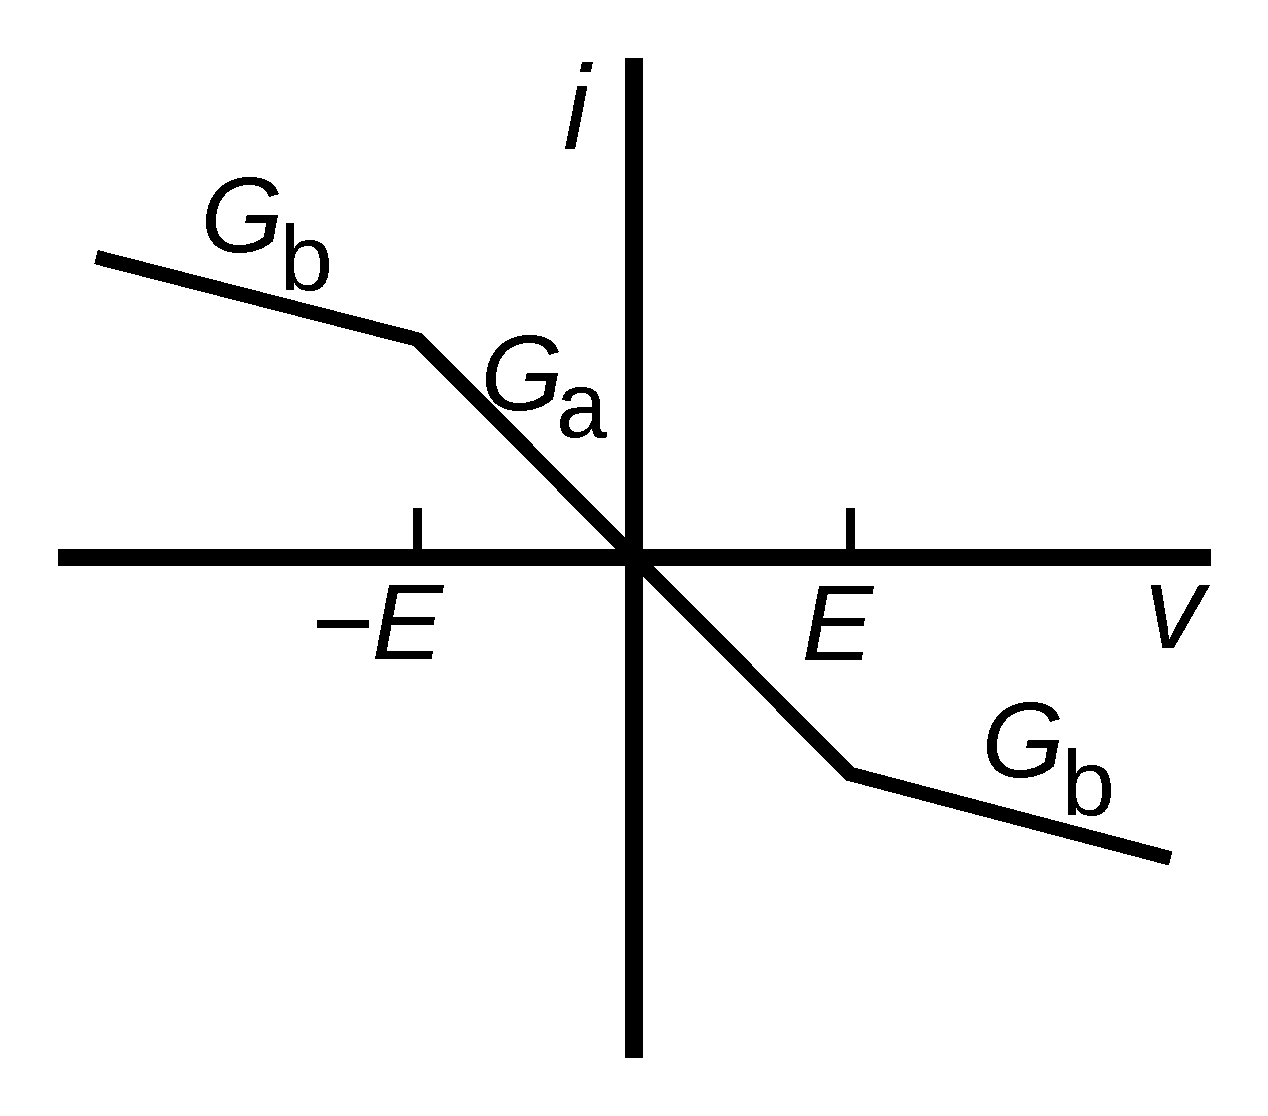
\includegraphics[width=0.49\textwidth]{chua-circuit/Chua-diode-characteristic-curve.pdf}
\caption[The chua circuit]{The chua circuit with its special chua diode. The chua diode is a piecewise-linear resistor with the characteristics as shown in the right figure.}
\label{figure:chuacircuit}
\end{figure}
\todo[inline]{Extend chua circuit caption.}

Using Kirchhoff's circuit laws to derive the equations of the chua circuit, we find the following nonlinear ordinary differential equations with the variables x(t), y(t) and z(t).

\begin{align*}
\frac{dx}{dt}&=\alpha [y-x-f(x)] &\frac{dx}{dt}\text{ is the voltage across the capacitor }C_1\\
RC_2\frac{dy}{dt}&= (x-y+Rz) &\frac{dy}{dt}\text{ is the voltage across the capacitor }C_2\\
\frac{dy}{dt}&=\beta (x-y+Rz) &\text{with } \frac{1}{RC_2} \text{ being }\beta\\
\frac{dz}{dt}&=-\gamma y &\frac{dz}{dt}\text{ is the current across the inductor }L_1\\
f (x) &= \frac{m_1 x + (m_0 - m_1)}{2 (| x + 1 | -| x - 1 |)} &f(x)\text{ describes the response of the piecewise linear resistor}
\end{align*}

\begin{comment}
dx/dt = c1*(y - x - f (x)) // m0 : slope in outer region
    dy/dt = c2*(x - y + z)    // m1 : slope in inner region
    dz/dt = -c3*y         // b : Breakpoints
    f (x) = m1*x + (m0 - m1)/2*(| x + 1 | -| x - 1 |)
\end{comment}

The chua circuit was chosen as a model system of a chaotic controller because of its simple definition through the equations as well as its prior usage in simple limiter control in [Corron]. Corron et al. showed in two different chaotic circuits, namely the driven chaotic pendulum and the chua circuit, how appropriate simple limiters can be applied to each system so that the chaotic behavior of each unbounded system could be controlled into behavior of different periodicities. Important to mention is that the Chua Circuit is not meant to be a model for appropriate leg movement, but the goal is to show that using simple limiters to control an arbitrary chaotic system. The different periodicities generated by the system leading to periodic leg movement could form different gait. The change of the terrain representing a change of the simple limiters can lead to a change in periodic movement, thereby adaption to different environments occurs. 

\subsubsection{Simple limiter control in Mathematica}

Before the circuit is used as a chaotic controller, the Chua circuit was modelled in Mathematica to observe its original chaotic behavior and influence it by simple limiters to exhibit different periodicities. The figure \ref{figure:chaoticchuacircuit} shows the Chua circuit's multiscroll attractor when using initial conditions \([-1.5,0,0]\) without any limiter.

\begin{figure}[H]
\centering
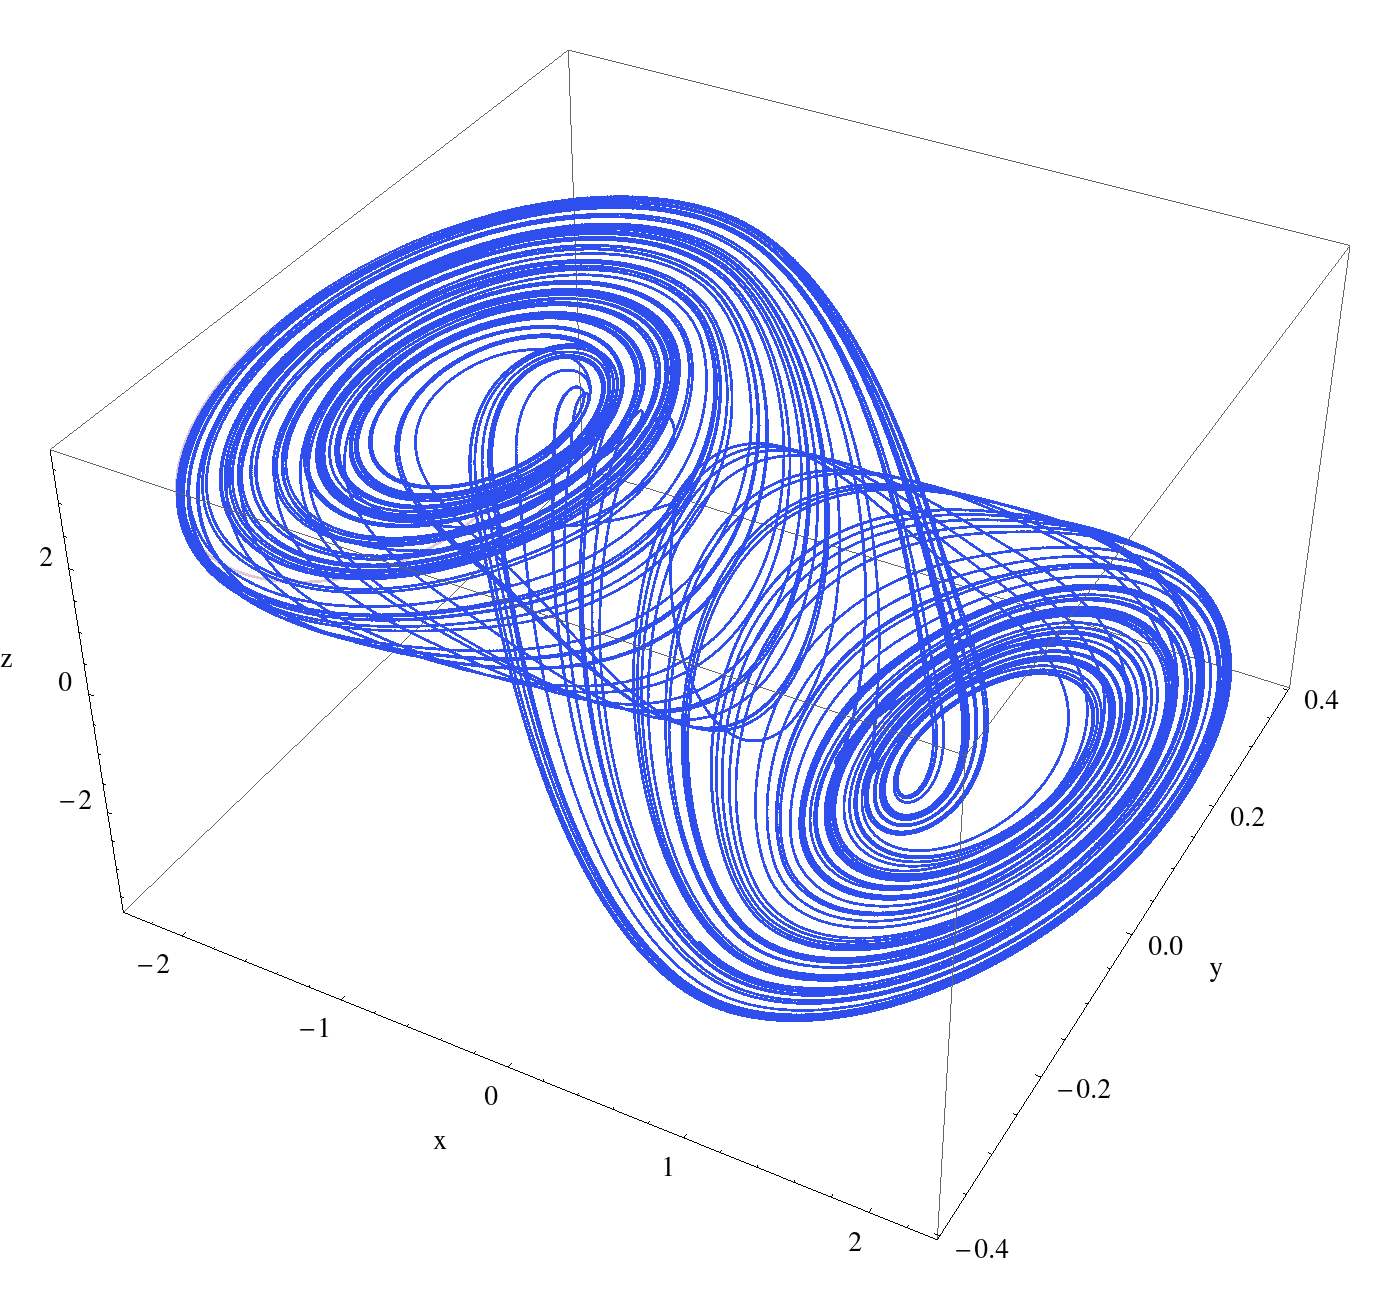
\includegraphics[width=0.8\textwidth]{chua-circuit/Unlimited-chua-circuit.png}
\caption[The multiscroll attractor]{The multiscroll attractor generated by the Chua's circuit without any simple limiter applied.}
\label{figure:chaoticchuacircuit}
\end{figure}

Then we introduce a simple soft limiter \[\text{softLim}(x) = \frac{1}{2} \left(\tanh\left(\frac{limitValue - x}{softness}\right) + 1\right)\] with the limiter response shown in figure \ref{figure:softlimiterresponse}.

\begin{figure}[H]
\centering
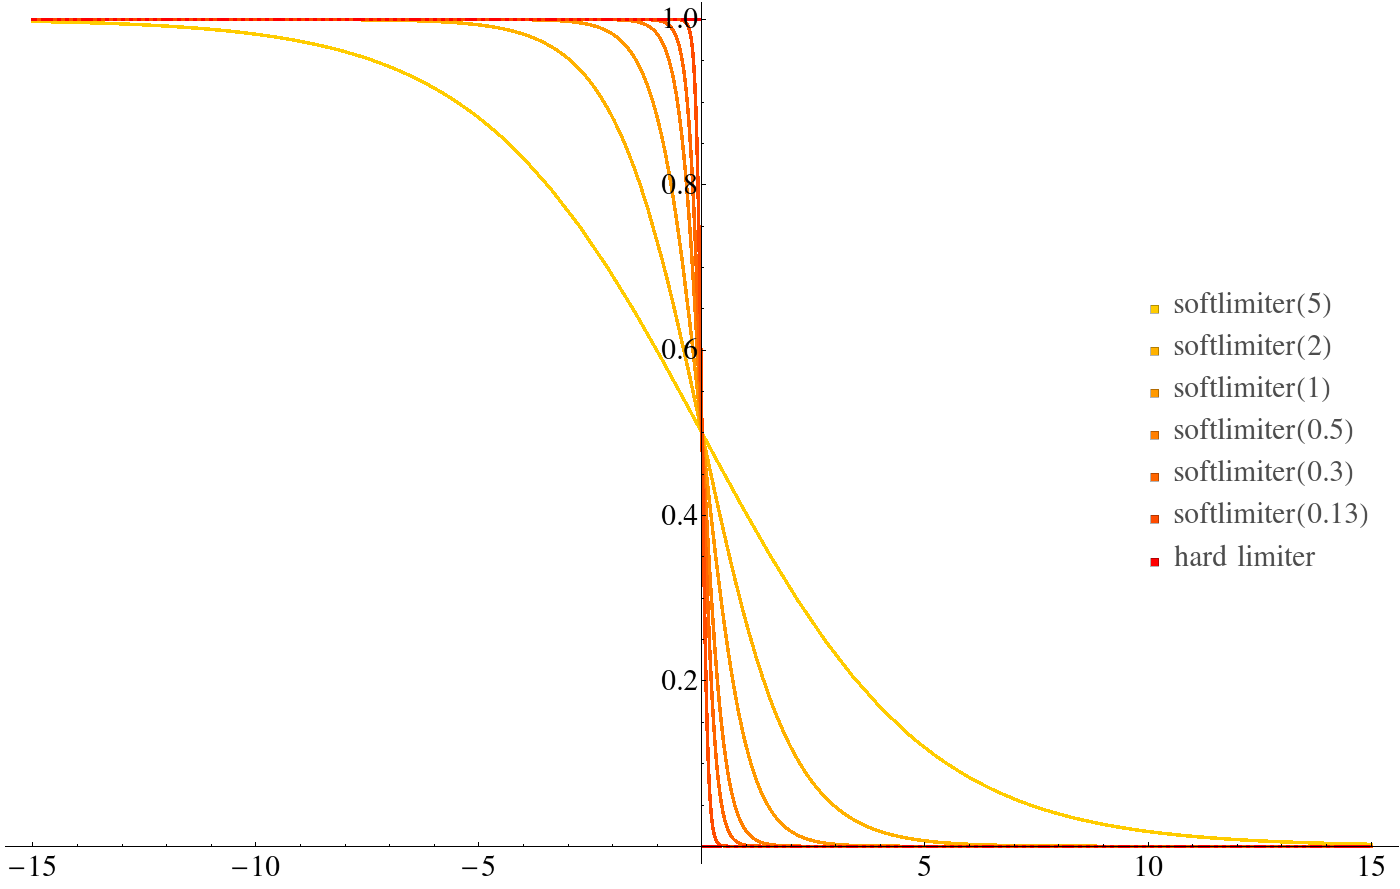
\includegraphics[width=0.8\textwidth]{chua-circuit/Limiter-softness-plot.png}
\caption[Soft limiter responses]{Soft limiter responses compared to the hard limiter response. The hard limiter response is shown in red. A trajectory approaching the 0 point from the negative side then runs into the limiter, so that the limiter is instantly fully applied. The soft limiter responses in orange on the other hand show that the limiter is applied more continuously. The softness values for the curves are 0.13, 0.3, 0.5, 1, 2 and 5. The curve with softness 0.13 approximates the hard limiter the best, the higher the value the softer the limiter gets applied. }
\label{figure:softlimiterresponse}
\end{figure}
\todo[inline]{Add different colors and a legend}

The limiter is added to the equations as shown below:

\begin{align*}
\frac{dx}{dt}&=\alpha [y-x-f(x)] \\
\frac{dy}{dt}&=\beta (x-y+Rz)\\
\frac{dz}{dt}&=-\gamma ~ y ~ \text{softLim}(x)\\
f (x) &= \frac{m_1 x + (m_0 - m_1)}{2 (| x + 1 | -| x - 1 |)}
\end{align*}

Initially a hard limiter defined as a piecewise function was chosen, however a soft limiter is a better model for physical limiters, because in physics, no hard limiters exist. Using the $softness$ parameter of the limiter, the softness of the limiter can be tuned where a \(softness = 10\) means very soft and a \(softness = 0.1\) means a very hard limiter. The $limitValue$ parameter defines the threshold value at which the limiter starts to be applied. We set the softness to a value of \(softness=0.13\) to approximate a rather hard limiter. With the above mentioned initial conditions, the trajectory in state space stays within the bounding box of \(x \in [-2.8717,2.2417],~y \in [-0.380467,0.386978],~z \in [-3.59156,3.62959]\).\\
If we now change the $limitValue$ parameter from \(>3.19\) which corresponds to no limiter influence to the trajectory to a value within \(limitValue \in [2.4,3.19[\), we can observe different chaotic trajectories. The limiter influences the circuit by limiting the change of current flow \(\frac{dz}{dt}\) when \(x\) approaches the limiter.

\begin{figure}[H]
\centering
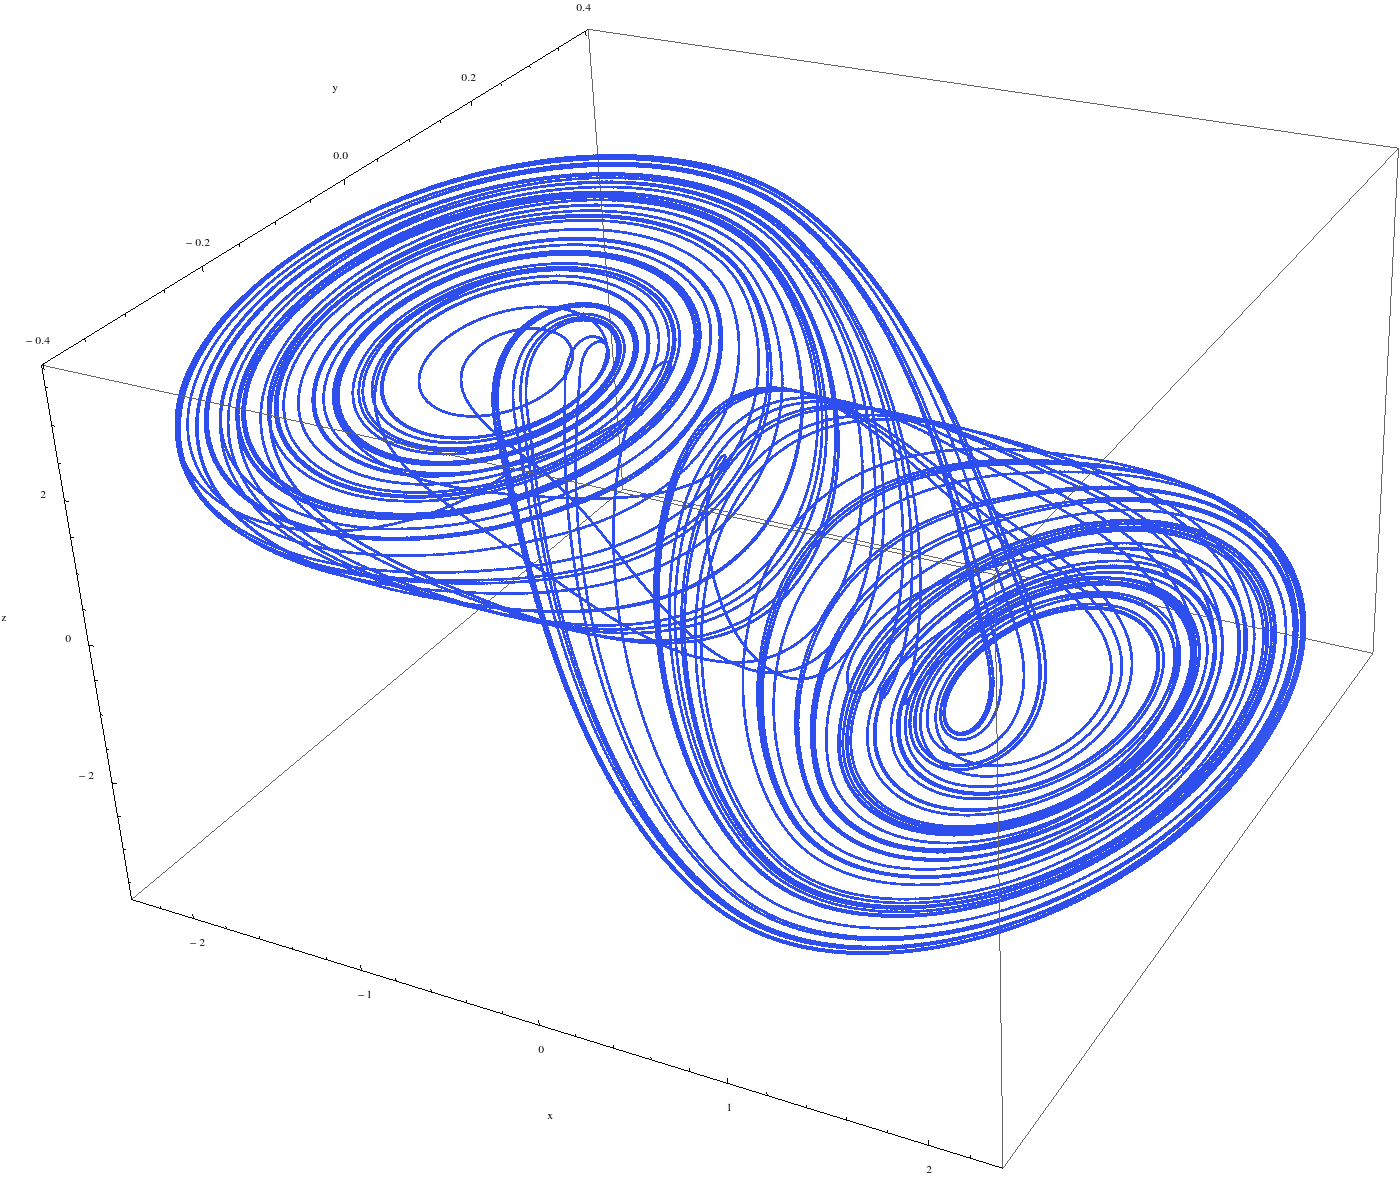
\includegraphics[width=0.8\textwidth]{chua-circuit/Limited-chua-circuit-2-5.png}
\caption[Figure of chaotic behaviors in range 2.4-3.19]{Figure of chaotic behaviors in range 2.4-3.19}
\label{figure:chaotictrajectories}
\end{figure}

When choosing a \(limitValue \in [2.28,2.4[\) one can observe that the limiter more and more suppresses chaotic behavior and reduces the number of times the trajectory switches back into the uppermost scroll of the multiscroll.

\begin{figure}[H]
\centering
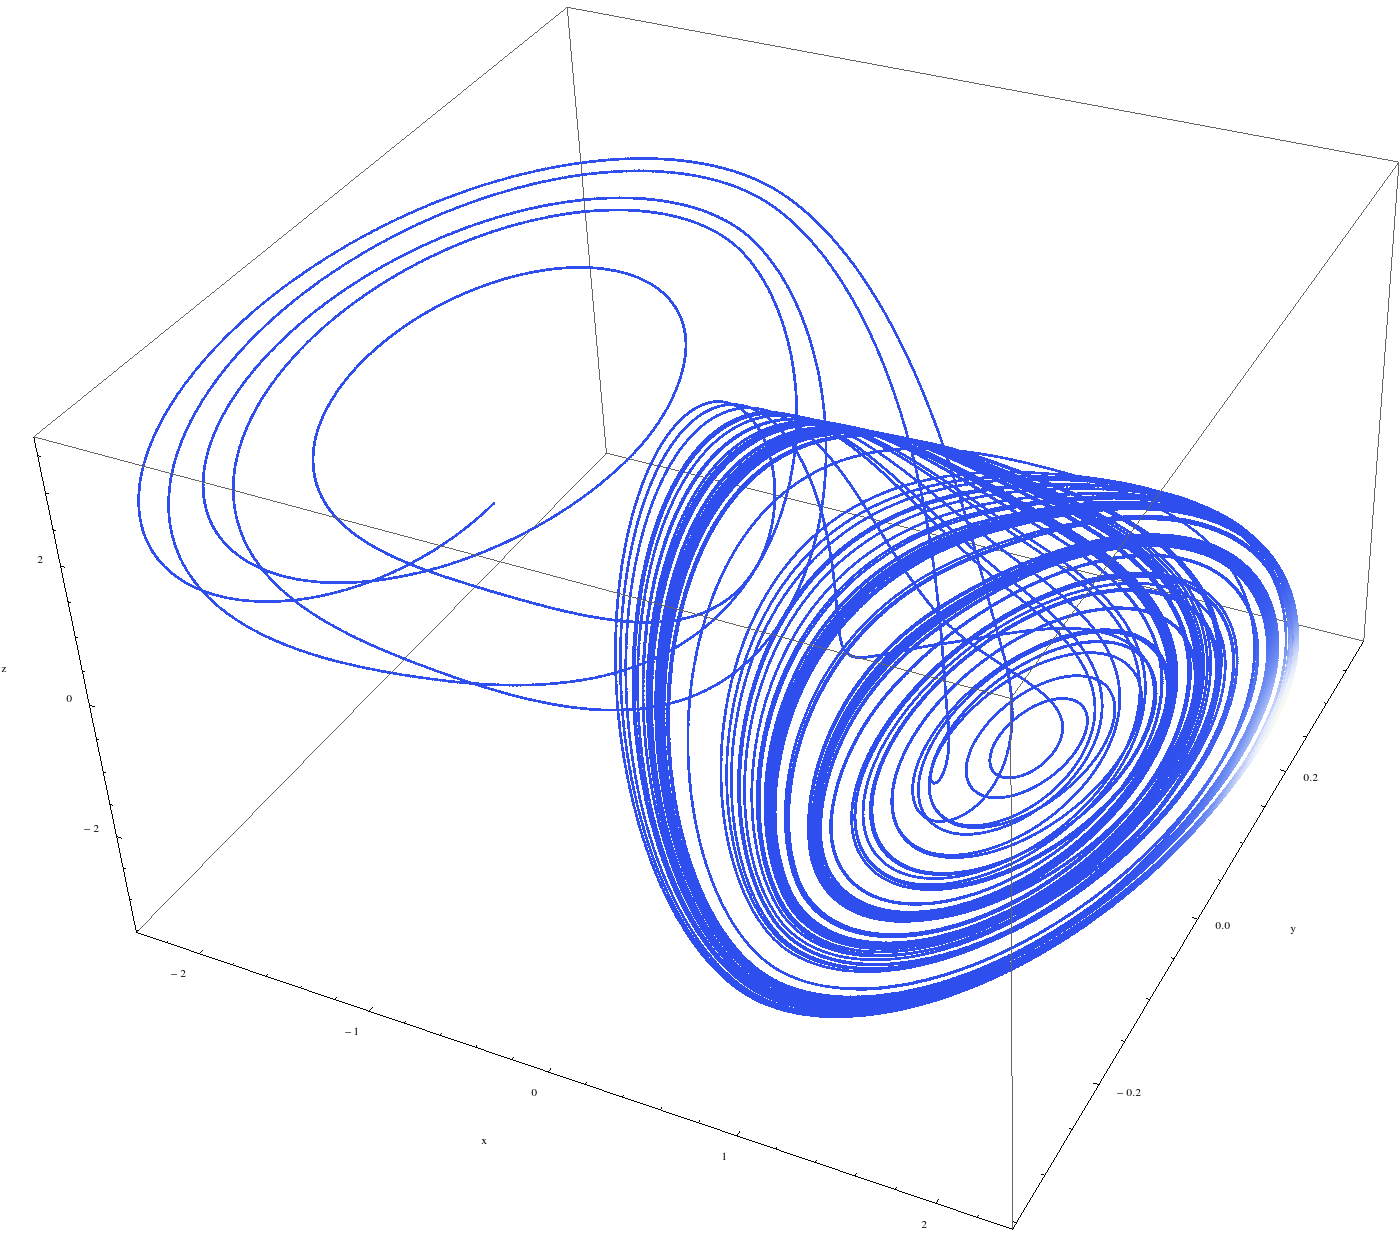
\includegraphics[width=0.8\textwidth]{chua-circuit/Limited-chua-circuit-2-28.png}
\caption[Figure of behaviors in range 2.28-2.4]{Figure of behaviors in range 2.28-2.4}
\label{figure:chaotictrajectories}
\end{figure}

With a value of \(limitValue \in [2,183, 2.28]\) the state only stays in the lowermost scroll and shows periodic behavior. The control behavior can be explained by looking at figure \ref{figure:chaoticchuacircuit} again. The trajectories that lead from the lower-most scroll to the upper-most scroll pass by at the outer orbits of the lower-most scroll and therefore have the highest x(t) values. The limiter is applied when a certain x(t) value is surpassed, therefore the limiter limits z(t) which then leads to a repelling influence from the limiter. The trajectory thereby is pulled back onto a former orbit, which stabilizes the state onto that orbit. The table \ref{table:periodicities} shows different limit values for different periodicities.

\begin{comment}
\begin{table}
\center
\begin{tabular}{|l|l|l|l|l|l|l|l|l|l|l|l|l|}
   \hline
   limitValue & 2.215 & 2.211 & 2.2105 & 2.2101 & 2.2101 &  2.208 & 2.207 & 2.206 & 2.205 & 2.1995 & 2.183 \\
   \hline
   Limit Cycle Period & 24 & 11 & 9 & 8 & 7 & 6 & 5 & 4 & 3 & 2 \\
   \hline
\end{tabular}
\caption{Whatever}
\label{table:periodicities}
\end{table}
\end{comment}

The plots below show the periodic trajectories for various limit values and a close-up look to make the period visible.

\begin{table}[H]
\renewcommand{\arraystretch}{1.2}
\center
\begin{tabular}{@{}ll@{}}
	\toprule
   \(limitValue\) & Limit Cycle\\
   \midrule
   2.215 & Period 24 \\ 
   2.211 & Period 11 \\
   2.21  & Period 10 \\
   2.209 & Period 9 \\
   2.208 & Period 8 \\
   2.207 & Period 7 \\
   2.206 & Period 6 \\
   2.205 & Period 5 \\
   2.2 & Period 4 \\
   2.1995 & Period 3 \\
   2.183 & Period 2 \\
   \bottomrule
\end{tabular}
\caption{Different limit values resulting in trajectories of different periodicity}
\label{table:periodicities}
\end{table}

{%
\setlength{\fboxsep}{0pt}
\setlength{\fboxrule}{1pt}

\hspace*{-0.2\textwidth}
\begin{minipage}{1.3\textwidth}
\begin{figure}[H]
\centering
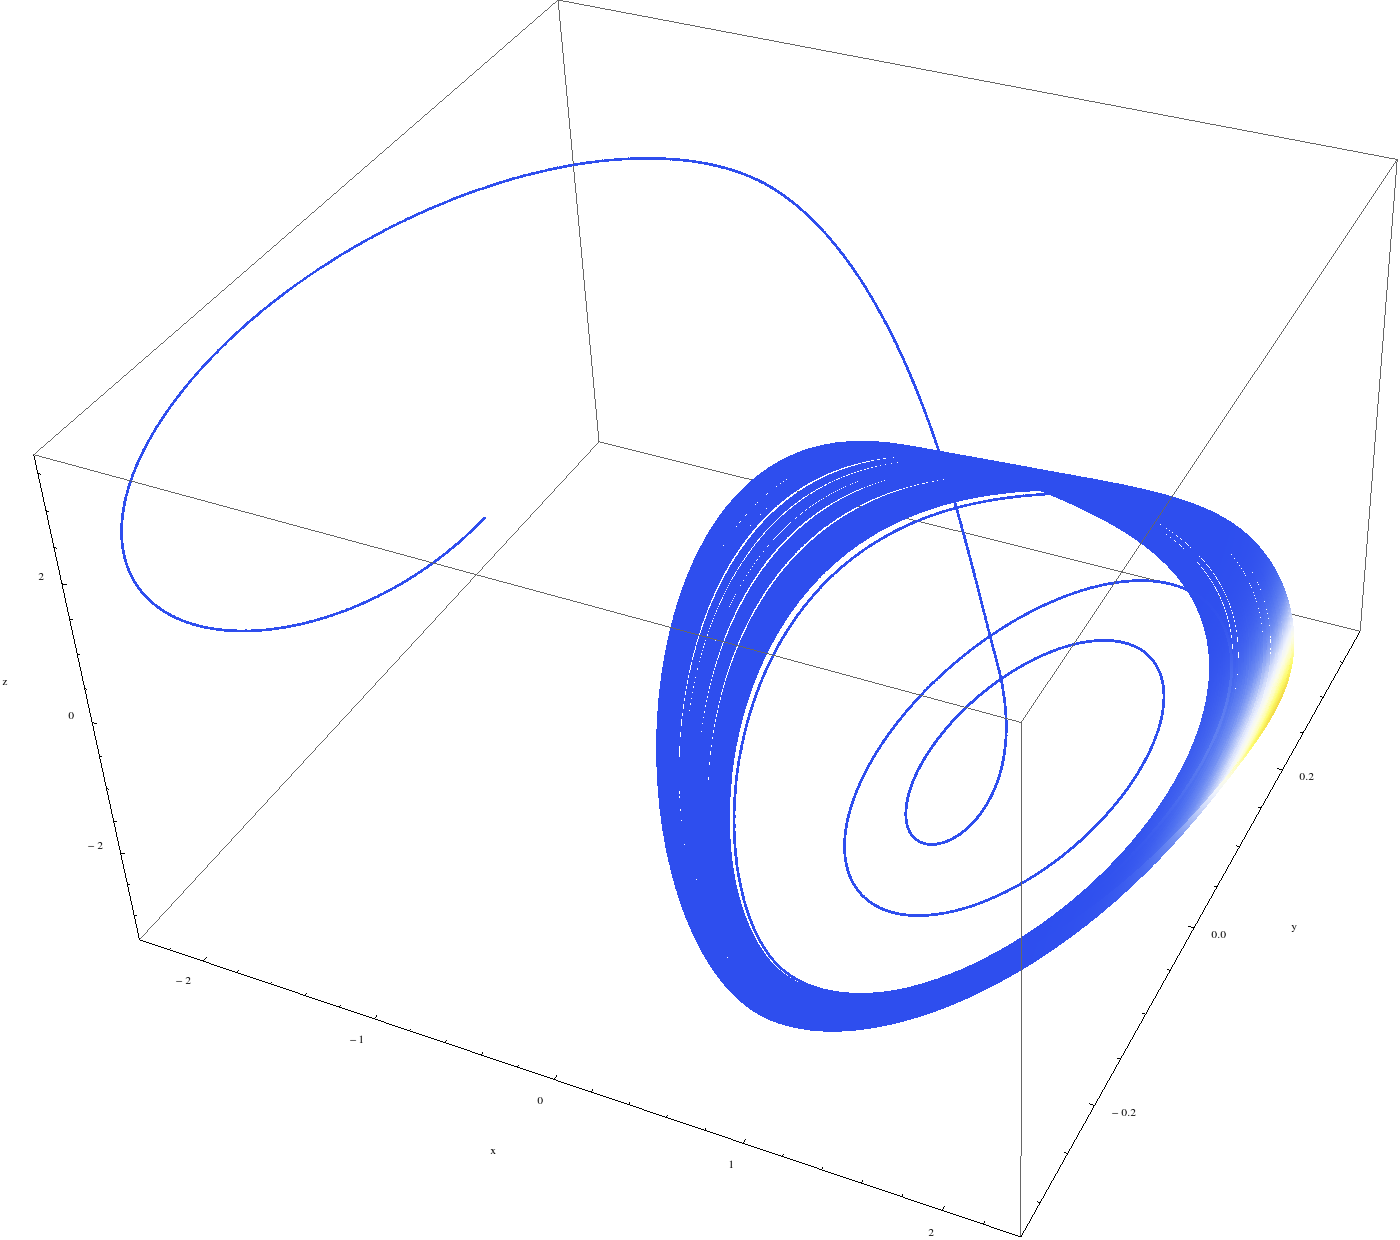
\includegraphics[width=0.48\textwidth]{chua-circuit/Limited-chua-circuit-2-215.png}
\fbox{
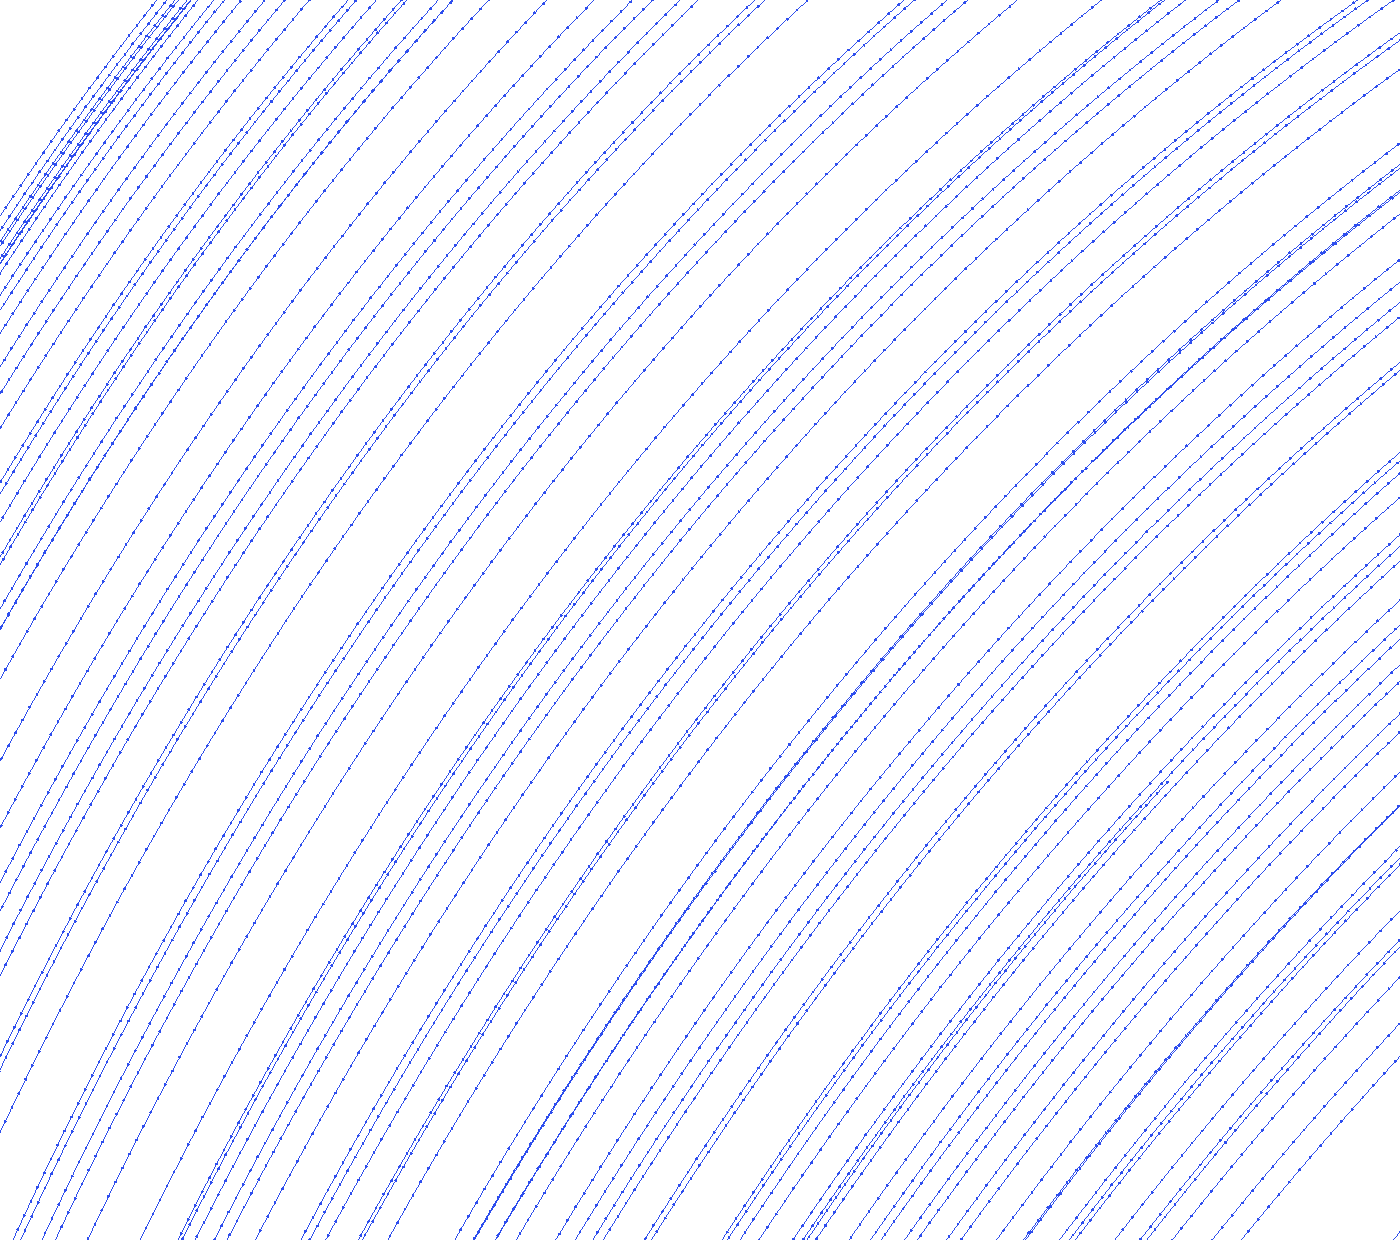
\includegraphics[width=0.48\textwidth]{chua-circuit/Limited-chua-circuit-2-215-closeup.png}
}
\caption[Figure of period 24 limit cycle]{Figure of period 24 limit cycle}
\label{figure:chaotictrajectories}
\end{figure}
\end{minipage}

\hspace*{-0.2\textwidth}
\begin{minipage}{1.3\textwidth}
\begin{figure}[H]
\centering
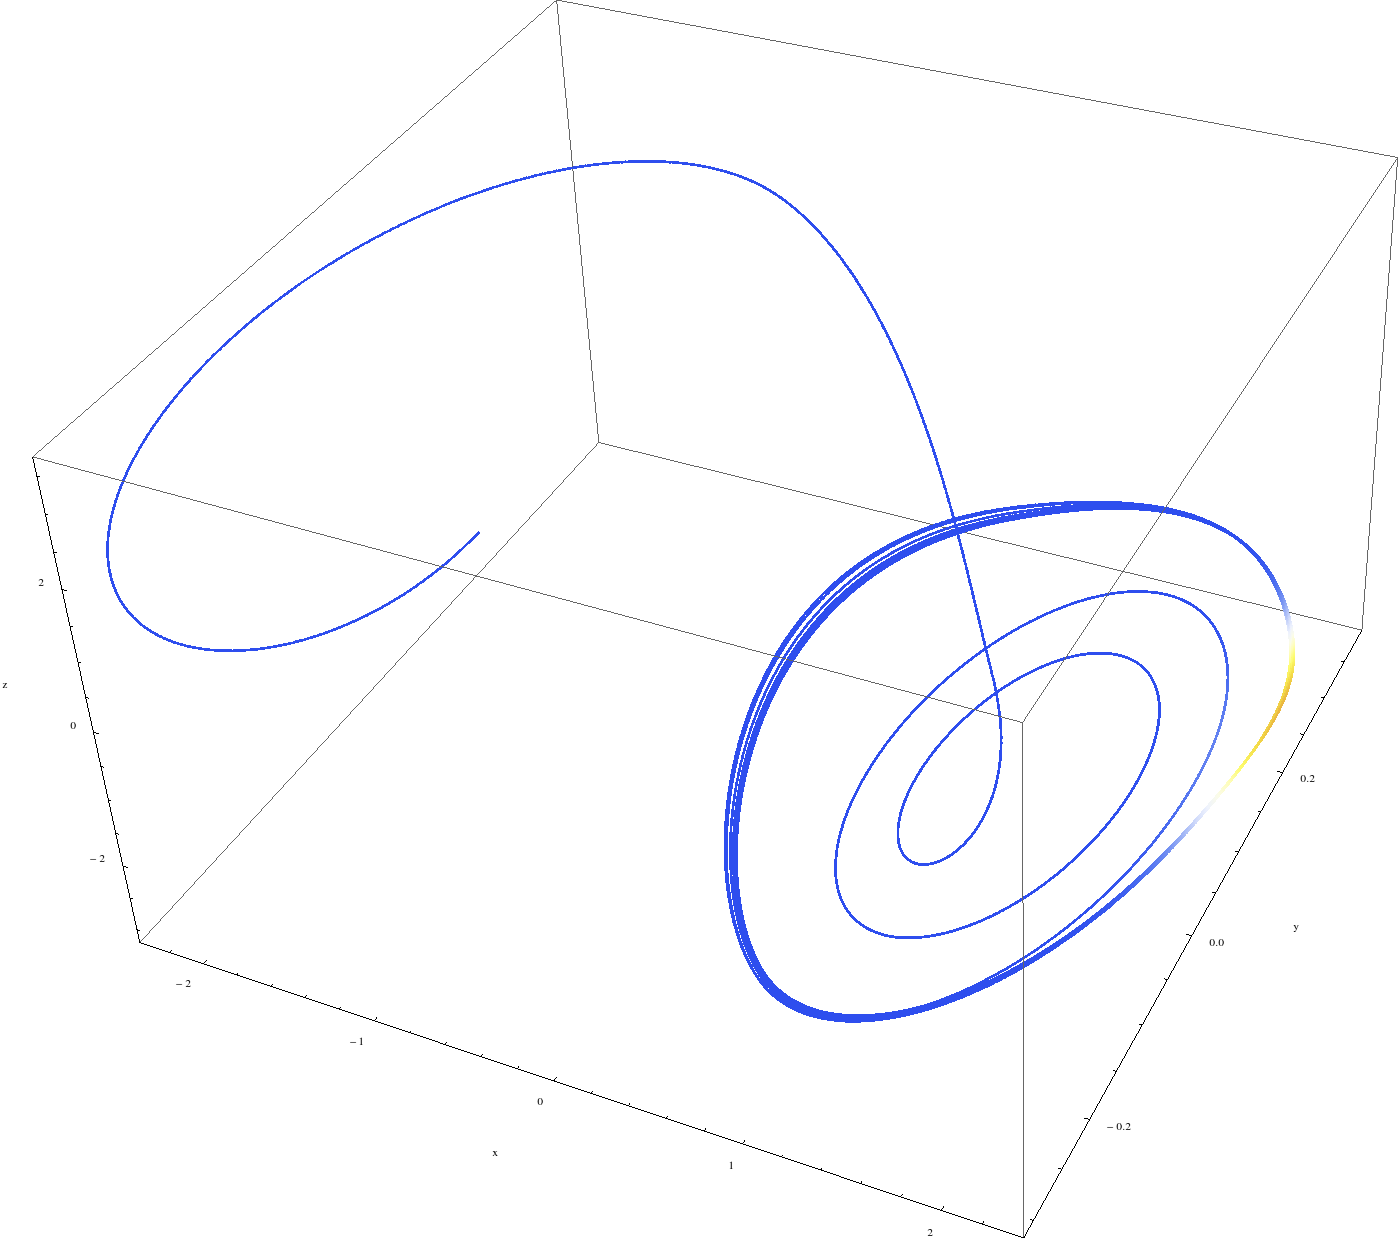
\includegraphics[width=0.48\textwidth]{chua-circuit/Limited-chua-circuit-2-21.png}
\fbox{

\includegraphics[width=0.48\textwidth]{chua-circuit/Limited-chua-circuit-2-21-closeup.png}
}
\caption[Figure of period 10 limit cycle]{Figure of period 10 limit cycle}
\label{figure:chaotictrajectories}
\end{figure}
\end{minipage}

\hspace*{-0.2\textwidth}
\begin{minipage}{1.3\textwidth}
\begin{figure}[H]
\centering
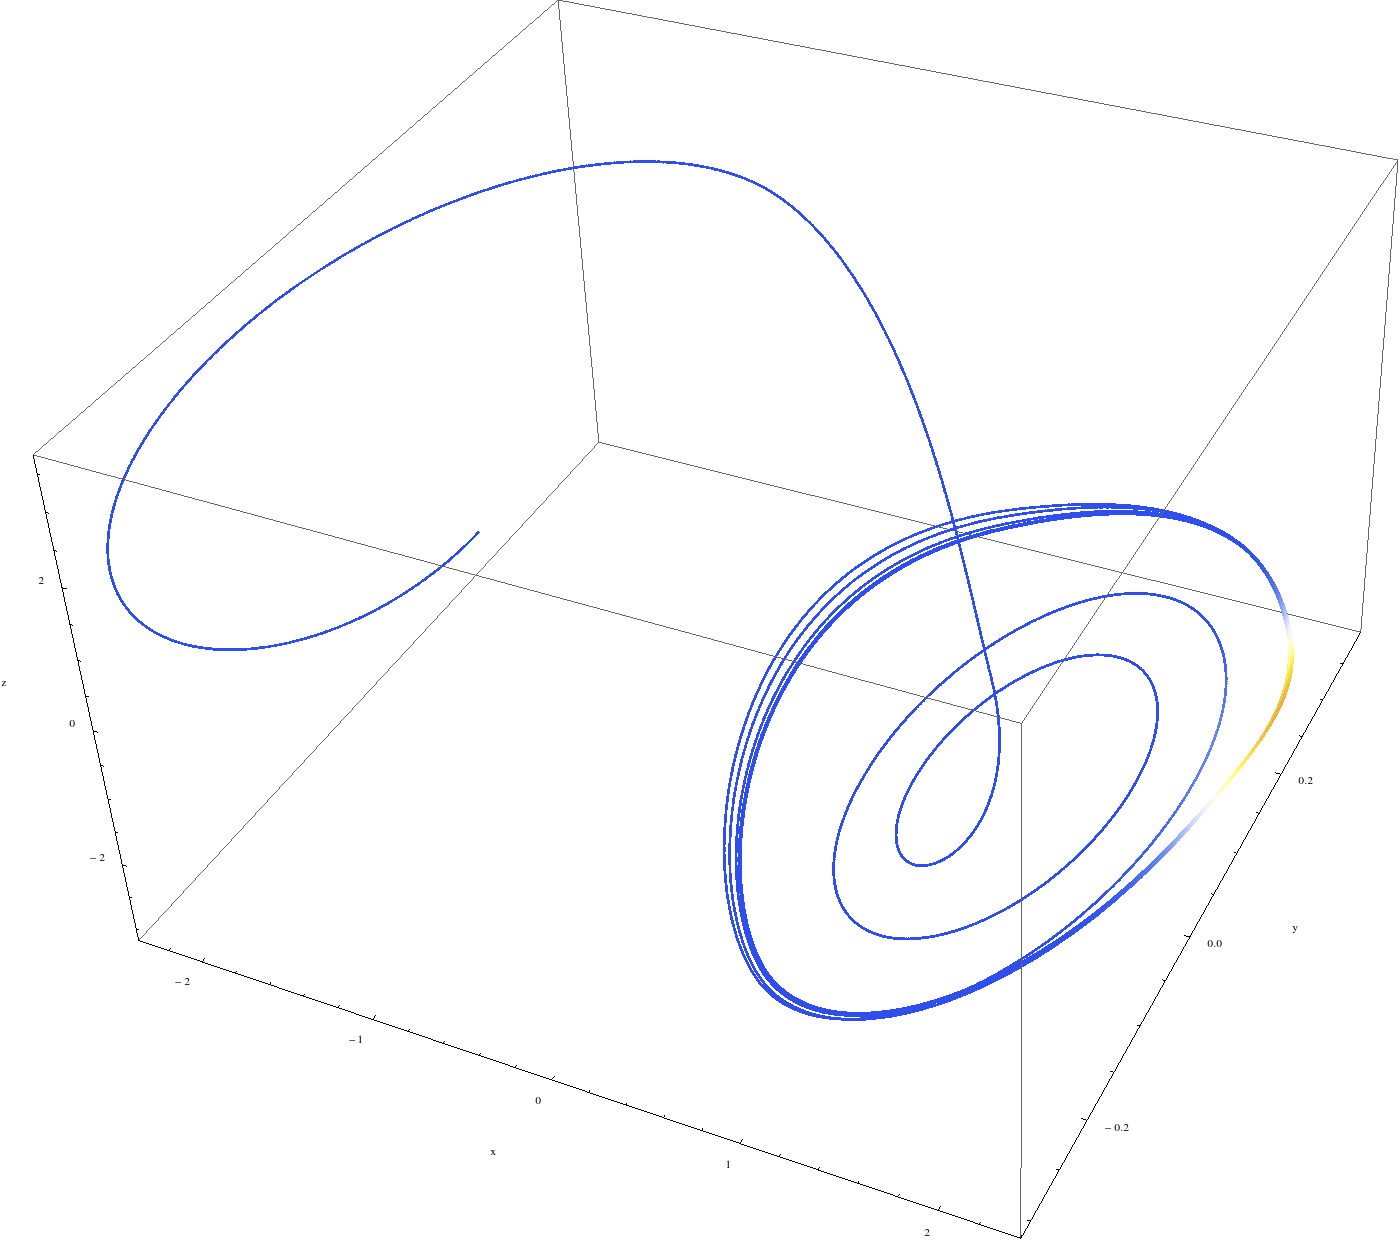
\includegraphics[width=0.48\textwidth]{chua-circuit/Limited-chua-circuit-2-207.png}
\fbox{

\includegraphics[width=0.48\textwidth]{chua-circuit/Limited-chua-circuit-2-207-closeup.png}
}
\caption[Figure of period 7 limit cycle]{Figure of period 7 limit cycle}
\label{figure:chaotictrajectories}
\end{figure}
\end{minipage}

\hspace*{-0.2\textwidth}
\begin{minipage}{1.3\textwidth}
\begin{figure}[H]
\centering
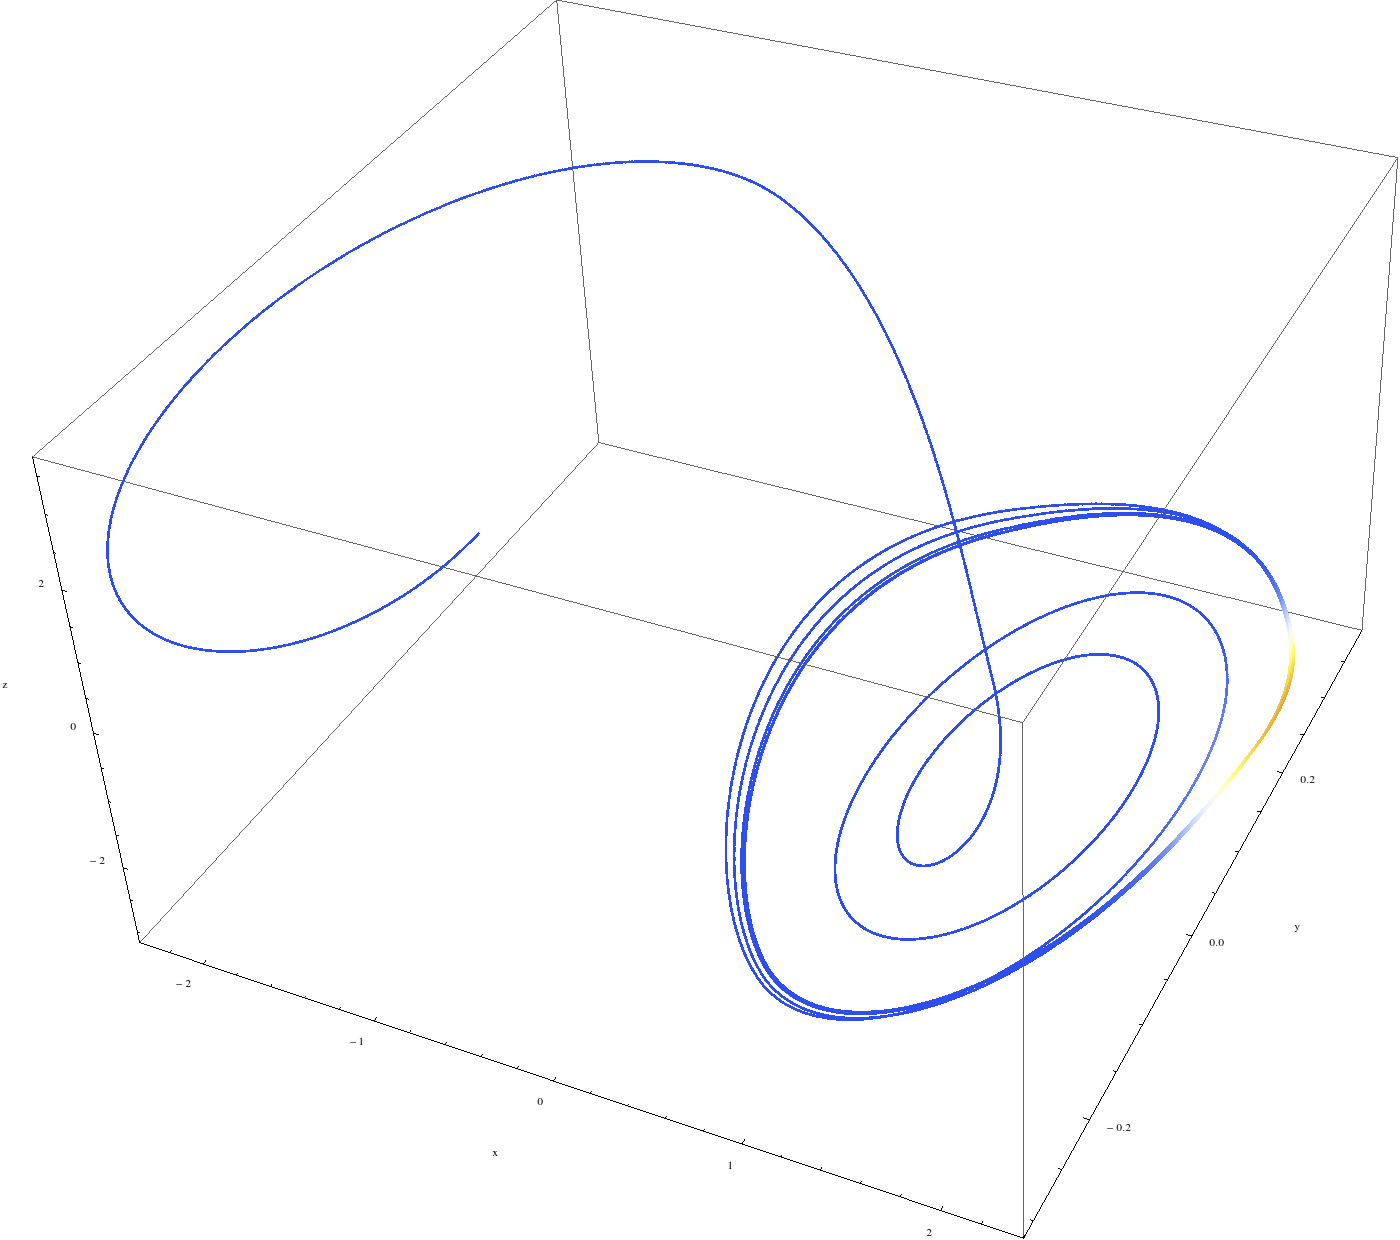
\includegraphics[width=0.48\textwidth]{chua-circuit/Limited-chua-circuit-2-205.png}
\fbox{
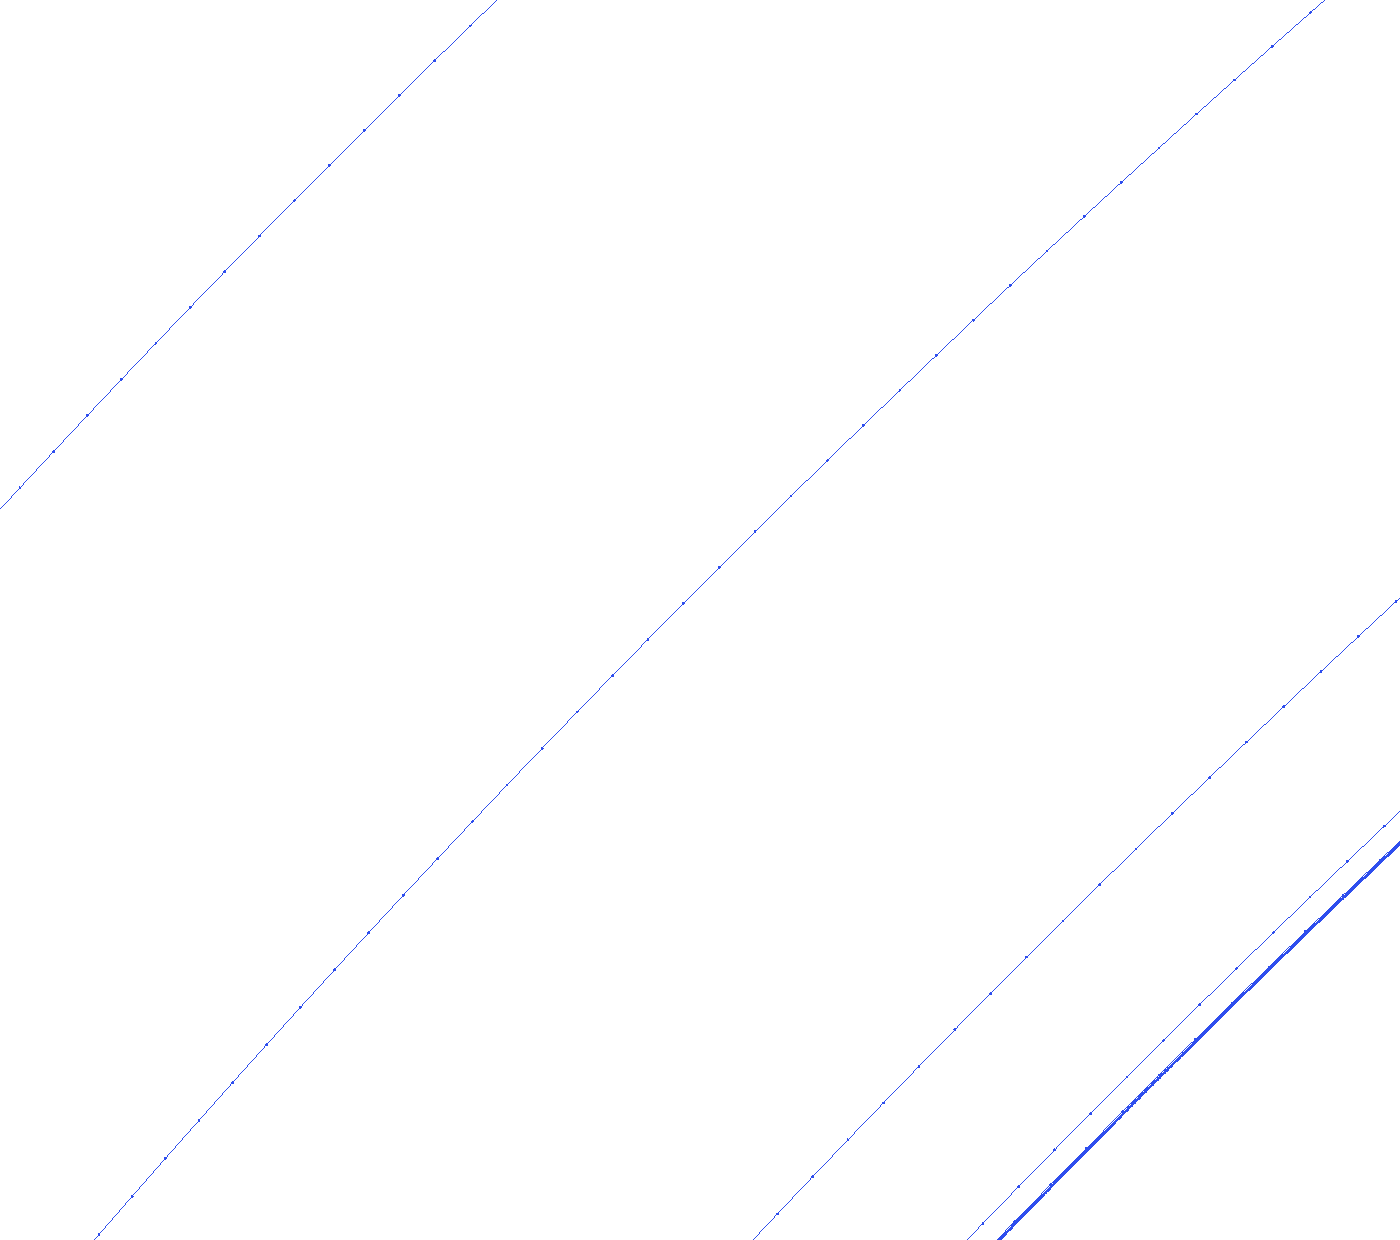
\includegraphics[width=0.48\textwidth]{chua-circuit/Limited-chua-circuit-2-205-closeup.png}
}
\caption[Figure of period 5 limit cycle]{Figure of period 5 limit cycle}
\label{figure:chaotictrajectories}
\end{figure}
\end{minipage}

\hspace*{-0.2\textwidth}
\begin{minipage}{1.3\textwidth}
\begin{figure}[H]
\centering
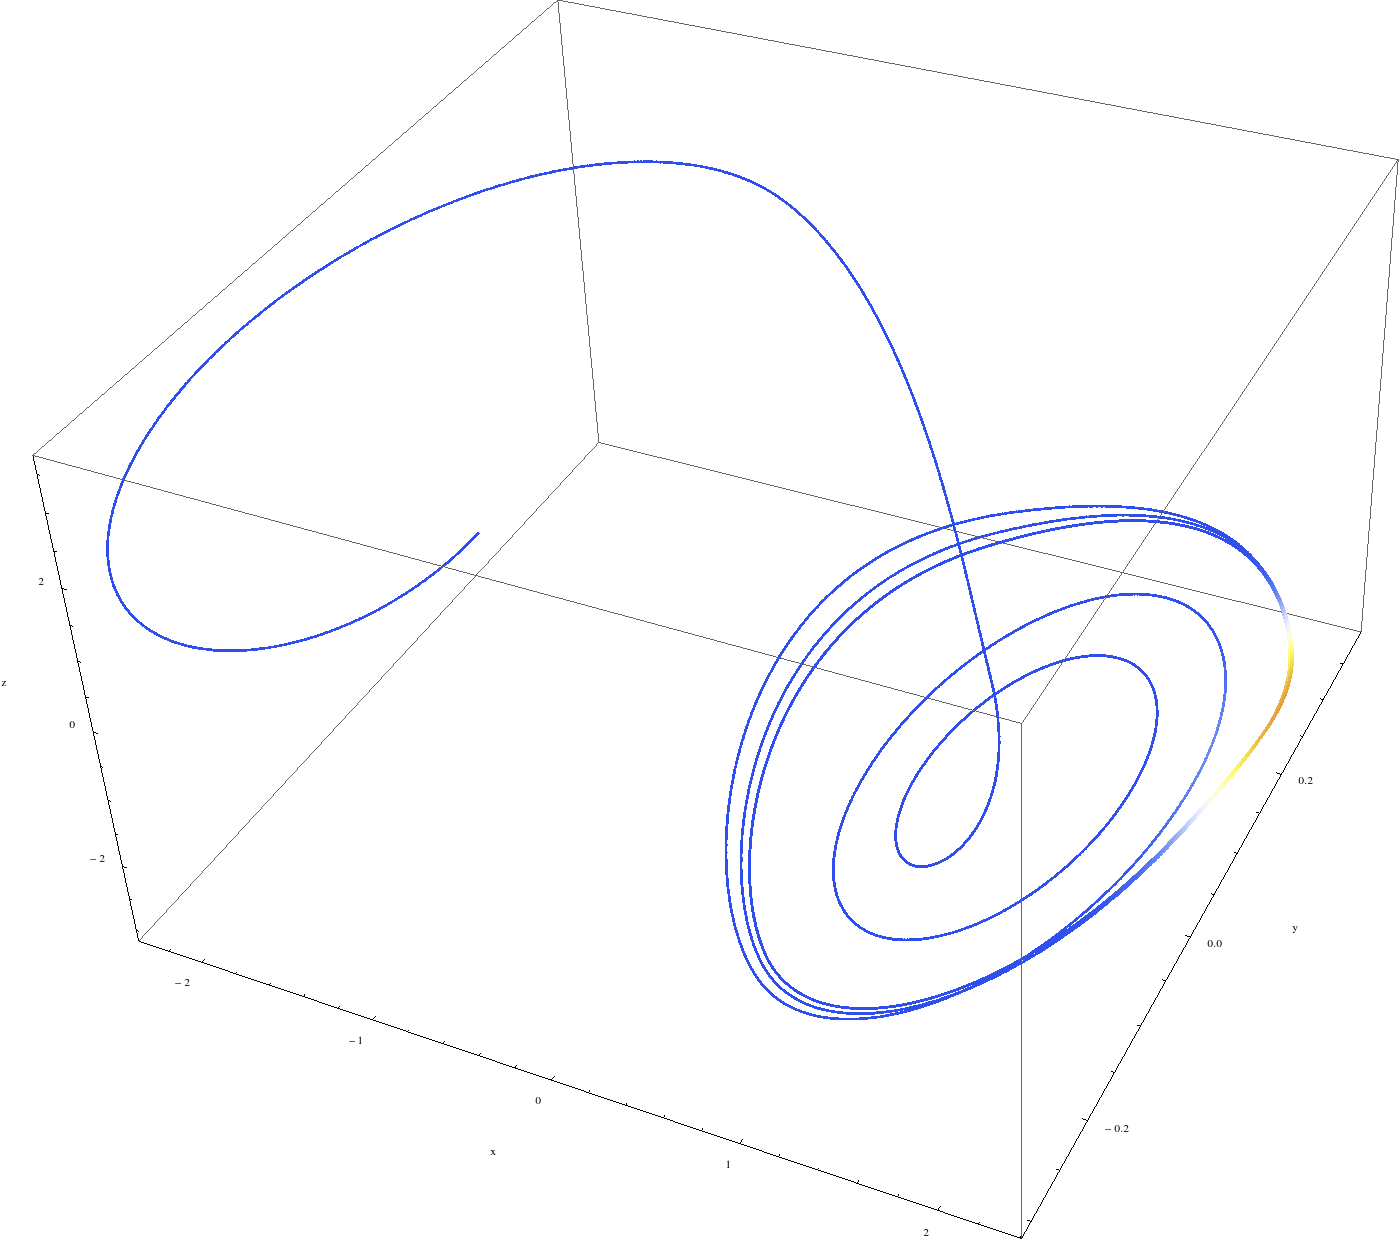
\includegraphics[width=0.48\textwidth]{chua-circuit/Limited-chua-circuit-2-1995.png}
\fbox{
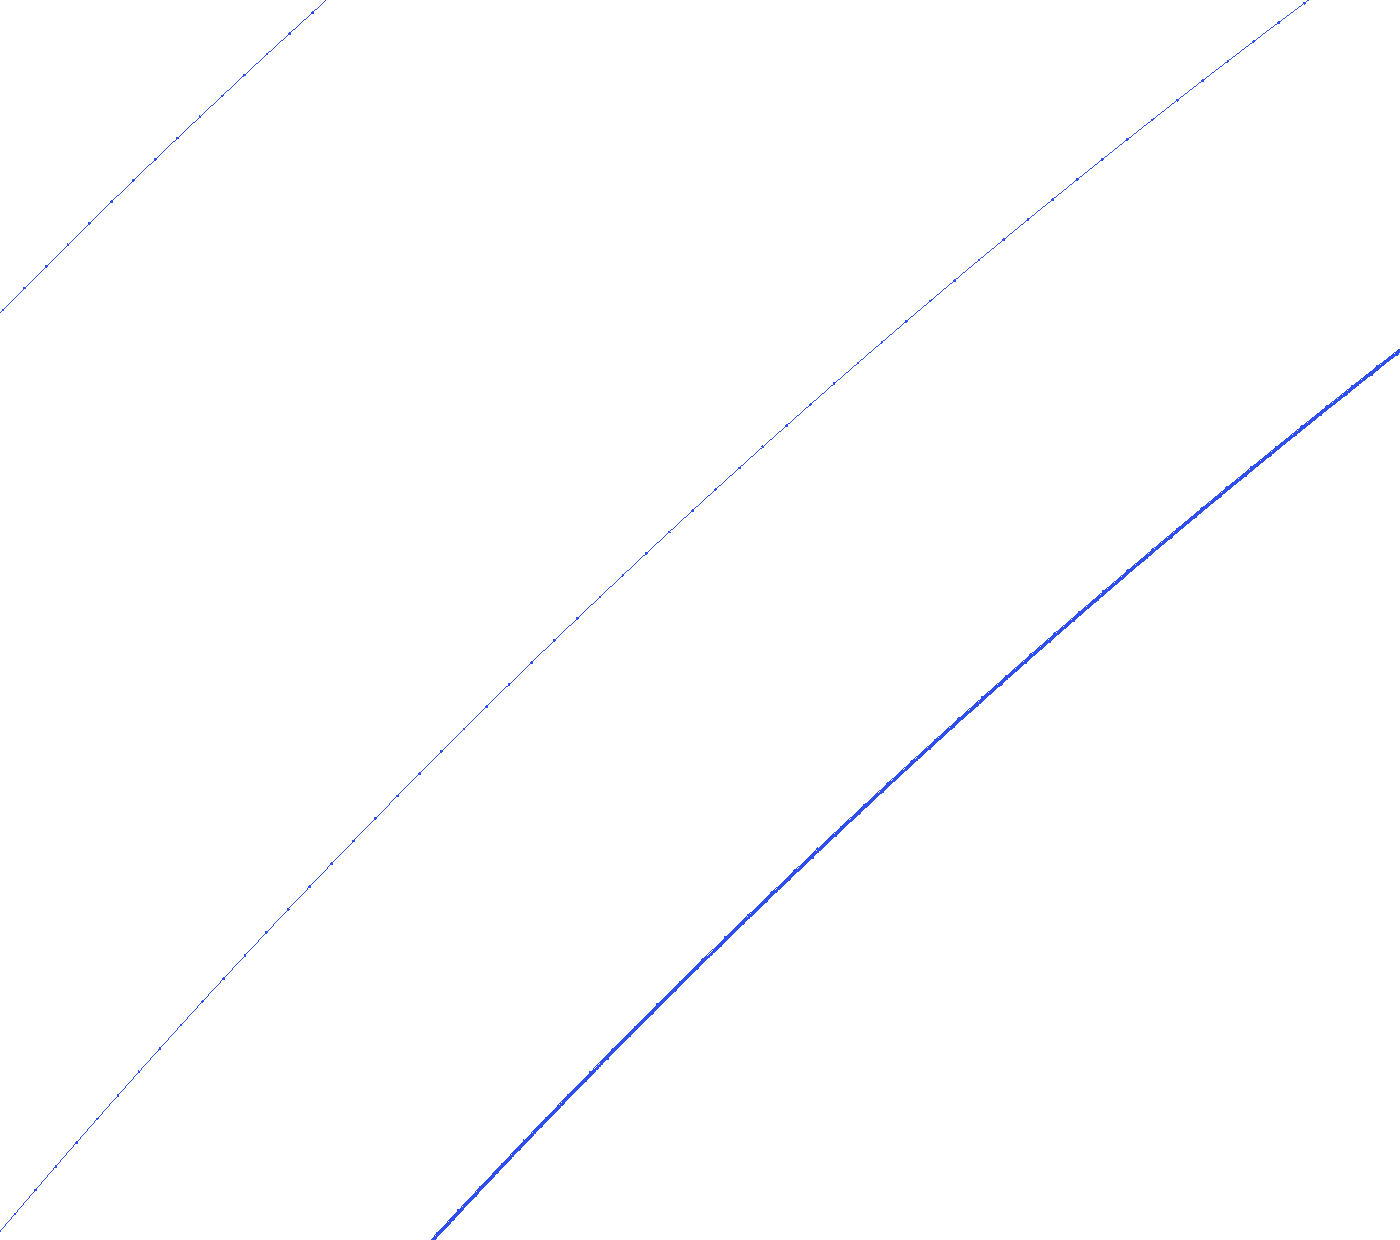
\includegraphics[width=0.48\textwidth]{chua-circuit/Limited-chua-circuit-2-1995-closeup.png}
}
\caption[Figure of period 3 limit cycle]{Figure of period 3 limit cycle}
\label{figure:chaotictrajectories}
\end{figure}
\end{minipage}

\hspace*{-0.2\textwidth}
\begin{minipage}{1.3\textwidth}
\begin{figure}[H]
\centering
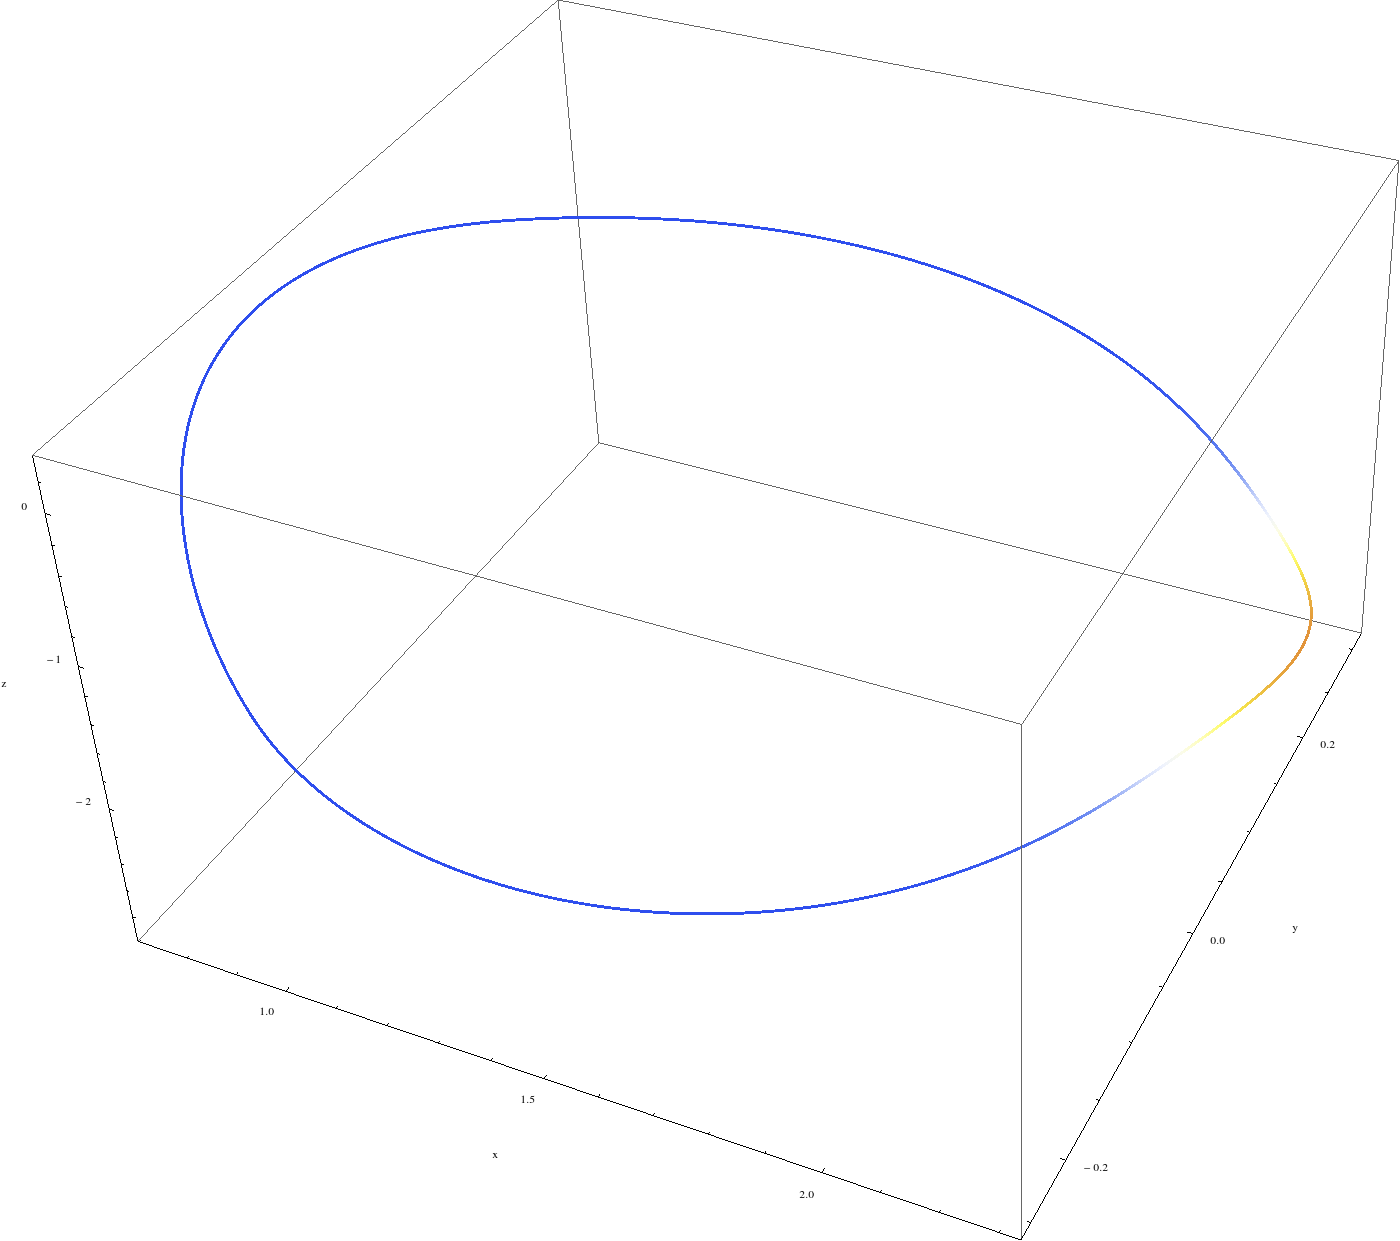
\includegraphics[width=0.48\textwidth]{chua-circuit/Limited-chua-circuit-2-183.png}
\fbox{
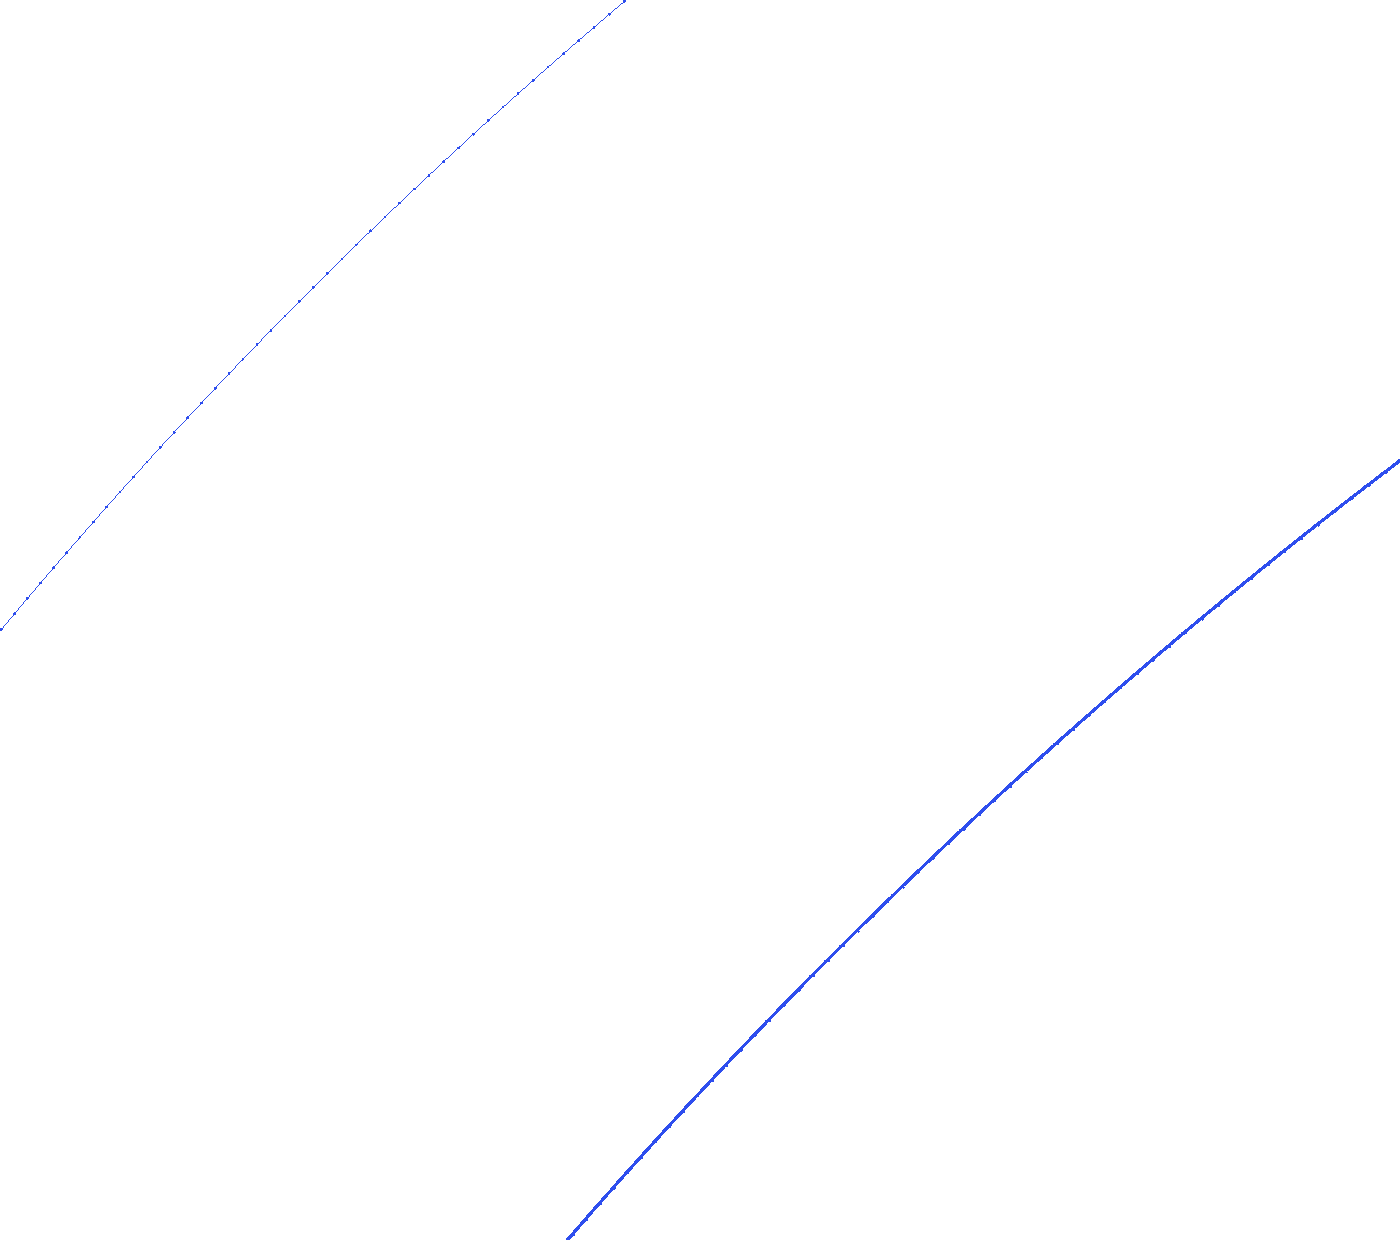
\includegraphics[width=0.48\textwidth]{chua-circuit/Limited-chua-circuit-2-183-closeup.png}
}
\caption[Figure of period 3 limit cycle]{Figure of period 2 limit cycle}
\label{figure:chaotictrajectories}
\end{figure}
\end{minipage}

From the table \ref{table:periodicities} it gets visible how densely packed the different periodicities are in the limiter space. The system is highly sensitive to the exact position of the limiter. But it gets more interesting as we move the limiter even further towards 0. Instead of showing a period 1 as one might expect, the periodicity becomes higher again for \(limitValue \in [2.183,2.15]\) and lowers again for \(limitValue \in [2.15,1.83]\). A self-similar pattern of increasing and decreasing periodicities can be observed.

\hspace*{-0.2\textwidth}
\begin{minipage}{1.3\textwidth}
\begin{figure}[H]
\centering
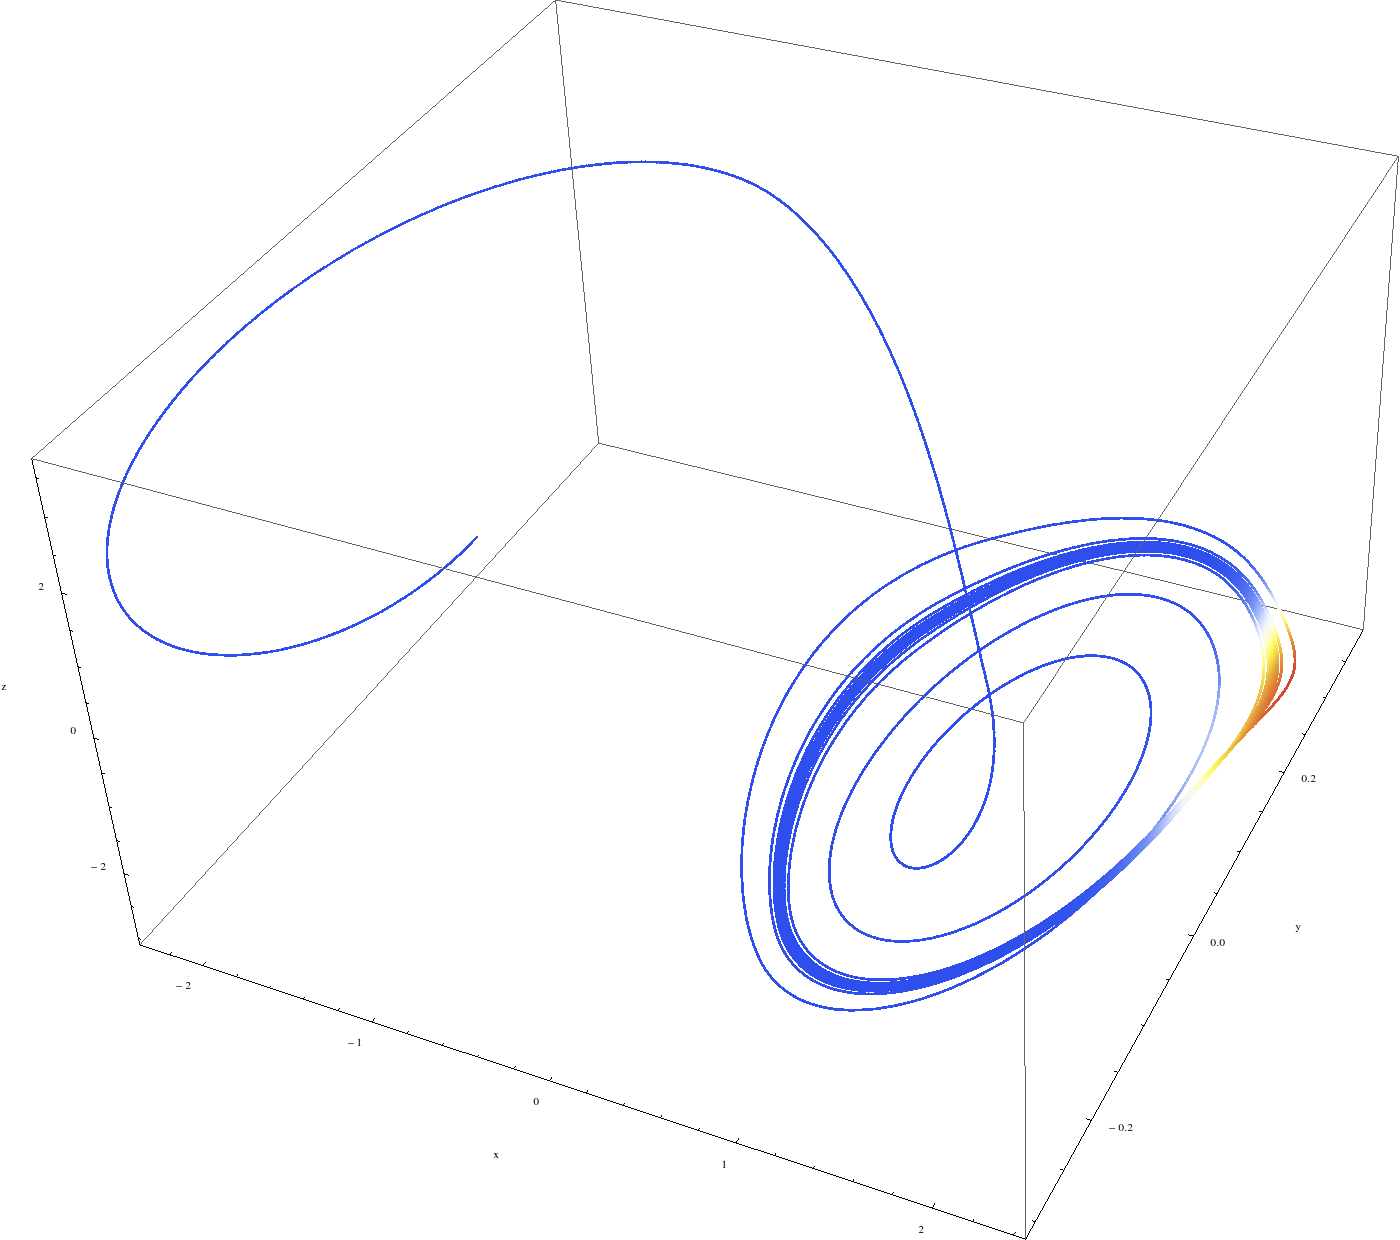
\includegraphics[width=0.48\textwidth]{chua-circuit/Limited-chua-circuit-2-15.png}
\fbox{
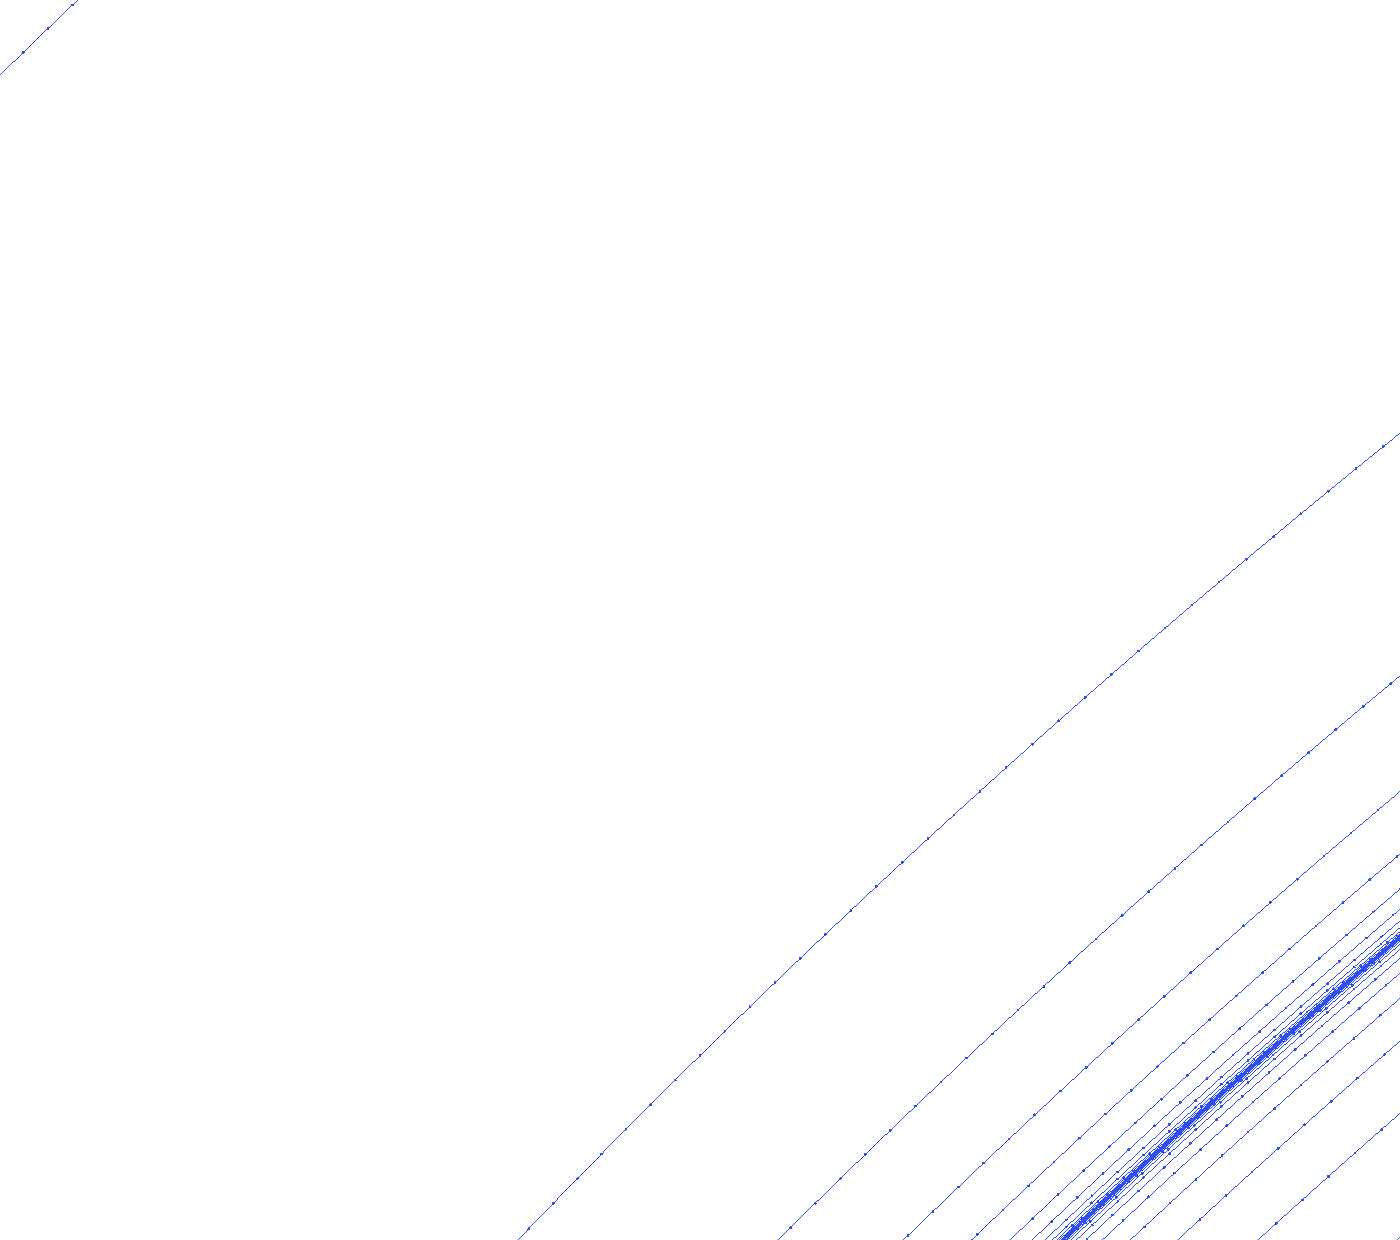
\includegraphics[width=0.48\textwidth]{chua-circuit/Limited-chua-circuit-2-15-closeup.png}
}
\caption[Figure of period 3 limit cycle]{Figure of very high period limit cycle}
\label{figure:chaotictrajectories}
\end{figure}
\end{minipage}

\hspace*{-0.2\textwidth}
\begin{minipage}{1.3\textwidth}
\begin{figure}[H]
\centering
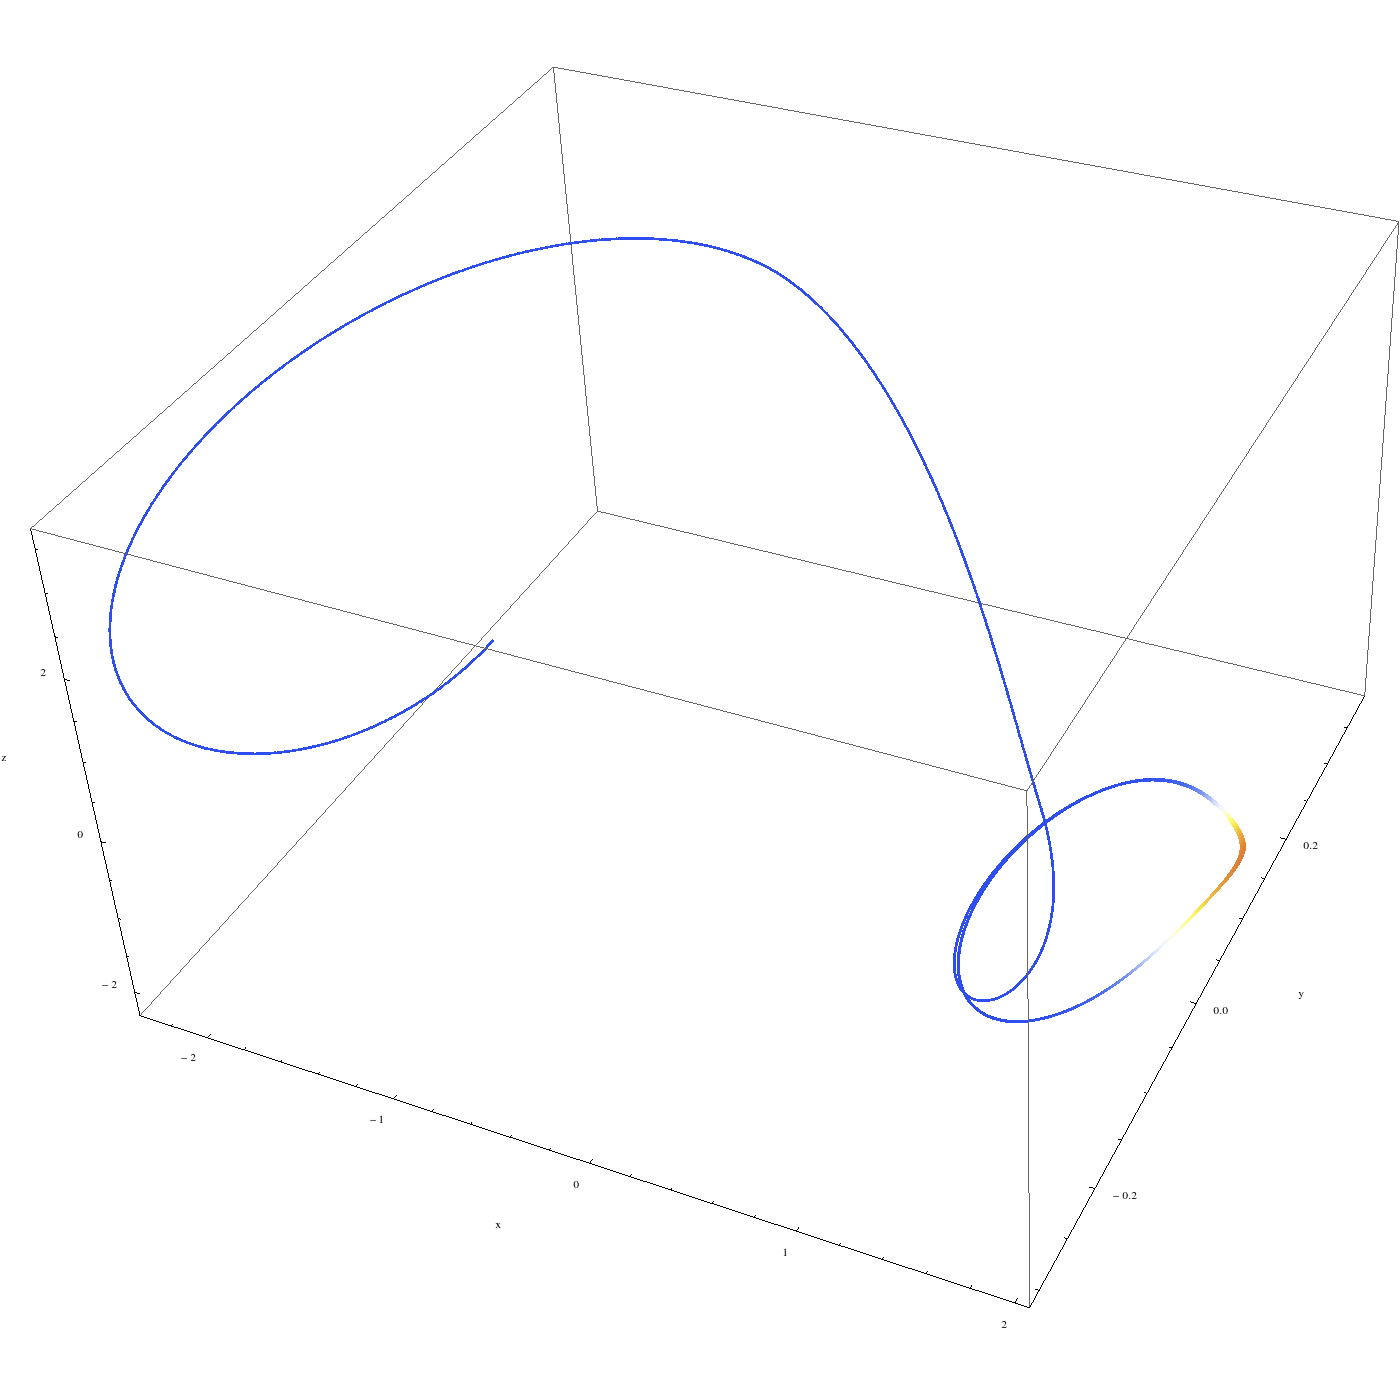
\includegraphics[width=0.48\textwidth]{chua-circuit/Limited-chua-circuit-1-83.png}
\fbox{
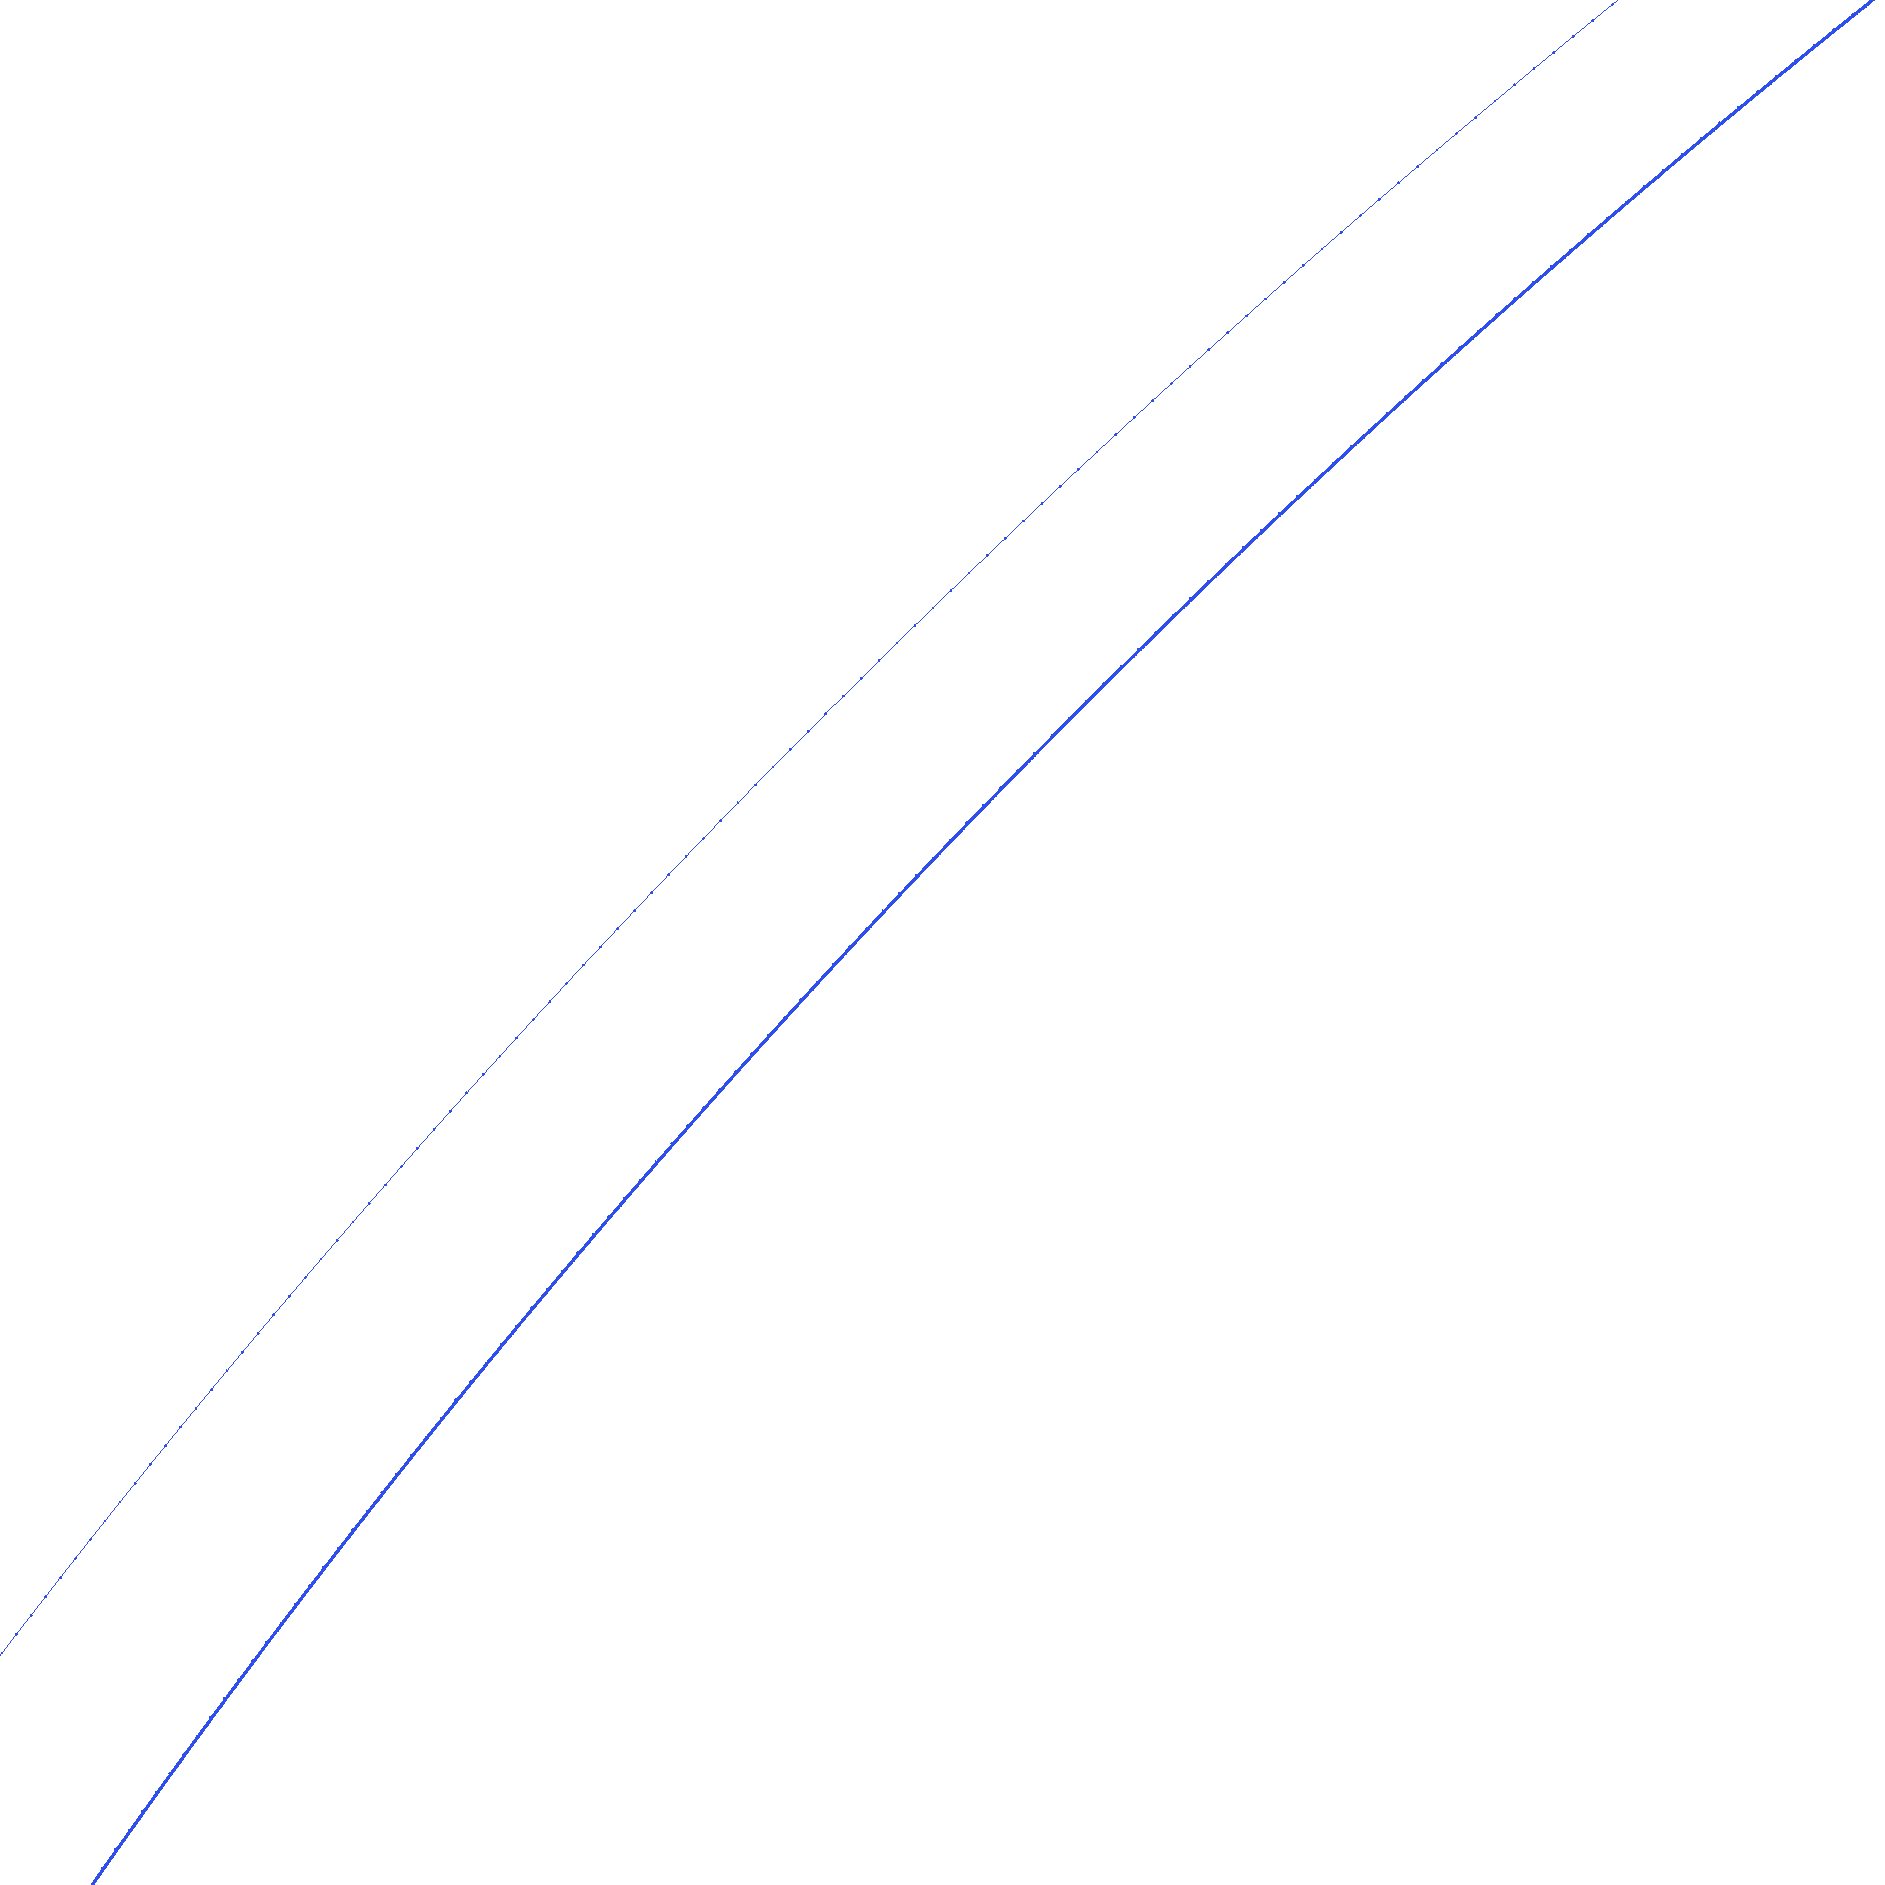
\includegraphics[width=0.48\textwidth]{chua-circuit/Limited-chua-circuit-1-83-closeup.png}
}
\caption[Figure of period 3 limit cycle]{Figure of period 1 limit cycle. The trajectory in the upper left half is the entry point to the periodic orbit before it gets limiter controlled.}
\label{figure:chaotictrajectories}
\end{figure}
\end{minipage}

}%

\end{document}